\chapter{Regularización y problema de Schrödinger}
\label{eot_sbp}

Si bien el problema de Kantorovich discreto \eqref{eq:kantorovich_discrete} es un problema de programación lineal (en particular, es convexo), es costoso de resolver por su cantidad cuadrática de incógnitas y nada garantiza la unicidad de la solución\footnote{Si bien se puede tener múltiples minimizadores, el valor mínimo es único, por lo que la no unicidad no influye sobre el valor de la distancia de Wasserstein entre dos distribuciones. Sin embargo, sí puede generar problemas al intentar aproximarla numéricamente.}, la cual en general no se tiene cuando el problema presenta cierto tipo de simetrías. Además, aun cuando la formulación dual \eqref{eq:kantorovich_dual_discrete} logra disminuir el número de incógnitas a una cantidad lineal, no soluciona el problema de la no unicidad de la solución, lo cual puede generar problemas al momento de resolver numéricamente el problema de optimización, ya sea el primal o el dual. Por otra parte, tal como se mencionó al final del \autoref{ot} el problema de transporte óptimo sufre de la maldición de la dimensionalidad al intentar aproximar la distancia de Wasserstein mediante una aproximación empírica, lo que limita fuertemente su uso en altas dimensiones.

Motivado por estas limitaciones, en \cite{cuturi2013sinkhorn} se propuso una técnica de regularización para el problema de Kantorovich, la cual posteriormente resultó ser equivalente a la formulación estática del puente de Schrödinger. La técnica de regularización entrópica consiste en agregar un término adicional a la función objetivo del problema de Kantorovich con el fin de poder obtener un problema dual que se pueda resolver eficientemente y que, además, caracterice la solución del problema primal.

\section{Transporte óptimo entrópico}
\label{eot_sbp/regularized}

Una forma de reparar el problema de la no unicidad de la solución es regularizar el problema de Kantorovich agregando un término conveniente que transforme la función objetivo en una función estrictamente convexa, permitiendo garantizar la unicidad del minimizador. Es decir, el problema de optimización regularizado es de la forma

\begin{equation}
	\label{eq:eot_motivation_discrete}
	\inf_{P\in \Pi_d(\mu,\nu)} \sum_{i=1}^n \sum_{j=1}^m C_{ij}P_{ij} + \epsilon \cdot\operatorname{Regularizador}(P),
\end{equation}

en el caso discreto y

\begin{equation}
	\label{eq:eot_motivation_continuous}
	\inf_{\pi\in \Pi(\mu,\nu)} \int_{\xspace\times\yspace} c(x,y)\d\pi(x,y) + \epsilon \cdot\operatorname{Regularizador}(\pi),
\end{equation}

en su versión continua. En ambos casos, $\epsilon>0$ es un ponderador que indica cuánta importancia se le da al regularizador durante la optimización. Recordando que el problema de Kantorovich define una distancia en (un subconjunto de) $\probmeasure{\xspace}$ cuando $\xspace=\yspace\subset\R^d$ y $c(x,y)=\norm{x-y}^p$, este nuevo problema de optimización permite obtener una versión suavizada de la distancia de Wasserstein.

Para la elección de la función de regularización, es útil observar que las soluciones del problema de Kantorovich por lo general pueden ser muy inestables con respecto a pequeñas variaciones en las medidas $\mu$ y $\nu$ o en el funcional de costo $c$, lo cual se puede ver en la \autoref{fig:eot_sbp/ot_instability}. Dado que esto no es una propiedad deseable, se puede elegir un regularizador que además de ser estrictamente convexo, promueva soluciones estables, pudiendo interpretar los problemas regularizados \eqref{eq:eot_motivation_discrete} y \eqref{eq:eot_motivation_continuous} como un trade-off entre tener un plan de Kantorovich inestable y tener una plan de transporte sub-óptimo pero más estable a cambios en los parámetros del problema. En este caso, el regularizador también se puede entender como un regularizador sobre el modelo ya que evita el sobreajuste a los datos de entrenamiento y le entrega robustez al problema con respecto a la función objetivo, donde el término adicional puede ser considerado como una incertidumbre sobre el funcional de costo real. Por otra parte, en muchos casos donde se utiliza la distancia de Wasserstein (p.g. como función de pérdida en un modelo de aprendizaje automático) es suficiente tener una aproximación razonable, por lo que el sesgo inducido por el regularizador no afecta considerablemente a la utilidad de la métrica de Wasserstein.

\insertimage{eot_sbp/ot_instability}{0.5}{Inestabilidad del mapa de Kantorovich bajo pequeñas perturbaciones en los parámetros del problema. En este caso, todos los elementos de $\xspace$ e $\yspace$ fueron perturbados con un ruido gaussiano de baja varianza. La imagen se encuentra en el archivo \texttt{ot\_instability.ipynb}.}

Como se verá en la siguiente subsección, una buena elección para el regularizador es la función de información media, la cual es estrictamente convexa y, además, promueve soluciones más suaves (en algún sentido a precisar). En particular, en el caso discreto, este regularizador forzará a que el plan de transporte entrópico óptimo sea denso, en el sentido de que todos los puntos en $\xspace=\{x_i\}_{i=1}^n$ envían masa a todos los puntos en $\yspace=\{y_j\}_{j=1}^m$, a diferencia de lo que se observa en muchos casos donde los planes de Kantorovich son \textit{deterministas} al estar asociados a mapas de Monge donde no se permite división de masa por parte de los elementos de $\xspace$. Además, como se verá en la \autoref{eot_sbp/static_sbp/sinkhorn}, este problema se puede resolver de forma eficiente, siendo esto último uno de los mayores beneficios del transporte óptimo entrópico (EOT).

\subsection{Regularización entrópica}
\label{eot_sbp/regularized/eot}

Para el problema de Kantorovich discreto \eqref{eq:kantorovich_discrete} se utilizará como regularizador (el negativo de) la función de entropía con el fin de promover una alta entropía del plan de transporte. Por otra parte, se verá que utilizar este regularizador es equivalente (salvo constantes aditivas) a regularizar el problema utilizando la divergencia de Kullback-Leibler (reversa) con respecto a la medida producto $\mu\otimes\nu$. Este último punto permitirá escribir el problema de transporte óptimo entrópico como un caso particular del problema del puente de Schrödinger en la \autoref{eot_sbp/static_sbp}.

\subsubsection{Problema entrópico discreto}

Para estudiar el problema de transporte óptimo entrópico se comenzará dando su formulación en un escenario discreto, donde $\xspace=\{x_i\}_{i=1}^n$ e $\yspace=\{y_j\}_{j=1}^m$ son conjuntos finitos que serán dotados de medidas discretas.

Se comenzará definiendo la entropía de una medida de probabilidad discreta:

\begin{defn}[entropía discreta]
	\label{defn:discrete_entropy}
	Para una medida discreta $\mu\in\probmeasure{\xspace}$ con vector de probabilidad $a\in\Sigma_n$, se define la entropía discreta de $\mu$ como:

	\begin{equation}
		\label{eq:discrete_entropy}
		\entropy{\mu} := - \sum_{i=1}^n a_i\log(a_i),
	\end{equation}

	donde, por continiuidad, se define $0\cdot\log(0)=0$ en el caso que algún $a_i\in[0,1]$ sea nulo.

\end{defn}

Dado que la medida discreta $\mu\in\probmeasure{\xspace}$ se identifica con el vector de probabilidad $a\in\Sigma_n$, es usual escribir $\entropy{a}$ en vez de $\entropy{\mu}$. Del mismo modo, dado que las medidas medidas $\mu\in\probmeasure{\xspace\times\yspace}$ se identifican con su matriz de probabilidades\footnote{En este caso, la suma en \eqref{eq:discrete_entropy} es sobre todos los elementos de la matriz de probabilidades $P$.} $P\in\matrixspace{n,m}{[0,1]}$ mediante $P_{ij}=\mu(\{(x_i,y_j)\})$ (ver \eqref{eq:coupling_identification}), se suele escribir $\entropy{P}$ en vez de $\entropy{\mu}$.

Se verá que esta función cumple las propiedades deseadas:

\begin{prop}
	\label{prop:discrete_entropy_properties}
	Las siguientes propiedades son ciertas:

	\begin{enumerate}
		\item La función de entropía discreta $\mu\mapsto \entropy{\mu}$ es estrictamente cóncava y, en consecuencia, el regularizador $\operatorname{Regularizador}(P)=-\entropy{P}$ es estrictamente convexo y el problema \eqref{eq:eot_motivation_discrete} tiene solución única.

		\item Dadas dos medidas discretas, $\mu\in\probmeasure{\xspace}$ y $\nu\in\probmeasure{\yspace}$, con vectores de probabilidad $a\in\Sigma_n$ y $b\in\Sigma_m$ respectivamente, el problema de optimización

		      \begin{equation}
			      \label{eq:entropy_maximizer}
			      \max_{P\in\Pi_d(\mu,\nu)} \entropy{P},
		      \end{equation}

		      es maximizado por la matriz $ab^\top\in\matrixspace{n,m}{[0,1]}$, la cual es la matriz de probabilidades asociada a la medida producto $\mu\otimes\nu\in\probmeasure{\xspace\times\yspace}$.
	\end{enumerate}
\end{prop}

\begin{proof}
	Para la primera proposición, se verá que la función de entropía discreta definida en \eqref{eq:discrete_entropy} tiene matriz hessiana definida negativa para toda medida $\mu\in\probmeasure{\xspace}$:

	\begin{equation*}
		\frac{\partial\mathcal{H}}{\partial a_i}(\mu) = -\parent{\log(a_i) + 1}
		\implies \frac{\partial^2\mathcal{H}}{\partial a_i a_j}(\mu) =
		\begin{cases}
			\frac{-1}{a_i} & \text{si } i=j     \\
			0              & \text{si } i\neq j .
		\end{cases}
	\end{equation*}

	Por lo tanto, $\operatorname{D}^2\parent{\entropy{\mu}} = \diag{\frac{-1}{a_1},\ldots,\frac{-1}{a_n}}$ y, así, todos los valores propios de $\operatorname{D}^2\parent{\entropy{\mu}}$ son negativos\footnote{Recordar que los valores propios de una matriz diagonal son precisamente los valores de su diagonal.}, por lo que la matriz es definida negativa para toda medida $\mu\in\probmeasure{\xspace}$.

	Para la segunda proposición, el problema de optimización con sus restricciones escritas de forma estándar es:

	\begin{alignat*}{3}
		\max_{P\in\matrixspace{n,m}{\R}} \quad & -\sum_{i=1}^n \sum_{j=1}^m P_{ij}\log(P_{ij}) &  &                                                  \\
		\text{s.a:} \quad                      & a_i - \sum_{j=1}^m P_{ij} = 0,\quad           &  & \forall i\in\{1,\ldots,n\}                       \\
		                                       & b_j - \sum_{i=1}^n P_{ij} = 0,\quad           &  & \forall j\in\{1,\ldots,m\}                       \\
		                                       & -P_{ij}\leq 0, \quad                          &  & \forall i\in\{1,\ldots,n\},\, j\in\{1,\ldots,m\}.
	\end{alignat*}

	Dado que el problema es convexo, se pueden utilizar las condiciones de Karush–Kuhn–Tucker (KKT) para identificar a un máximo. El lagrangiano del problema $L:\matrixspace{n,m}{\R}\times\matrixspace{n,m}{\R}\times\R^n\times\R^m\to\R$ es:

	\begin{equation*}
		L(P,\lambda,\kappa,\eta) =
		-\sum_{i=1}^n \sum_{j=1}^m P_{ij}\log(P_{ij})
		+ \kappa_i \parent{a_i - \sum_{j=1}^m P_{ij}}
		+ \eta_j \parent{b_j - \sum_{i=1}^n P_{ij}}
		+ \lambda_{ij}(-P_{ij}).
	\end{equation*}

	Las condiciones de KKT para este problema son:

	\begin{itemize}
		\item Factibilidad: $P \in\Pi_d(\mu,\nu)$
		\item Holgura complementaria: $\lambda_{ij}(-P_{ij})=0,\, \forall i\in\{1,\ldots,n\},\, j\in\{1,\ldots,m\}$
		\item $\lambda_{ij}\geq 0, \forall i\in\{1,\ldots,n\},\, j\in\{1,\ldots,m\}$.
		\item Punto crítico para el lagrangiano: $\nabla_P L = 0$.
	\end{itemize}

	Para que la última condición se cumpla es necesario que:

	\begin{equation*}
		\frac{\partial L}{\partial P_{ij}}(P,\lambda,\kappa,\eta) = -\parent{\log(P_{ij})+1} - \kappa_i - \eta_j - \lambda_{ij} = 0 \implies P_{ij} = e^{-1 - \kappa_i - \eta_j - \lambda_{ij}}.
	\end{equation*}

	Se verá que es posible encontrar una tripleta $(P,\kappa,\eta)$ que cumpla las condiciones de KKT cuando $\lambda_{ij}=0$. Bajo esta consideración, la última igualdad permite escribir $P_{ij}$ como un producto de la forma $P_{ij} = p_i q_j$ y así, para que la condición de factibilidad se cumpla es necesario que:

	\begin{align*}
		\sum_{j=1}^m P_{ij} = a_i \implies p_i \sum_{j=1}^m q_j = a_i \implies p_i = a_i \\
		\sum_{i=1}^n P_{ij} = b_j \implies q_j \sum_{i=1}^n p_i = b_j \implies q_j = b_j ,
	\end{align*}

	y, por lo tanto, con $P_{ij} = a_i b_j$ se cumplen todas las condiciones de KKT, por lo que $P=ab^\top$ es un máximo del problema.
\end{proof}

Por la proposición anterior, el mapa de transporte que maximiza la entropía en \eqref{eq:entropy_maximizer} es la medida producto $\mu\otimes\nu$ definida para cada par $(x_i,y_j)\in\xspace\times\yspace$ como

\begin{equation*}
	(\mu\otimes\nu)(\{x_i\}\times\{y_j\}) = \mu(\{x_i\})\,\nu(\{y_j\}) = (ab^\top)_{ij} = a_i b_j .
\end{equation*}

Este plan de transporte distribuye la masa de cada $x_i\in\xspace$ en todos los elementos de $\yspace$, donde cada $y_j\in\yspace$ recibe una cantidad proporcional a su masa $\nu(\{y_j\})=b_j$, por lo que la cantidad de masa transferida desde $x_i$ hacia $y_j$ (según $\mu\otimes\nu$) corresponde a $a_i b_j$. Recordando que en el caso discreto siempre se puede considerar que $a_i,b_j>0$, el plan de transporte $\mu\otimes\nu$ envía masa a todos los elementos de $\yspace$ desde todos los elementos de $\xspace$, siendo este el extremo opuesto a lo que realiza el mapa de Monge. Por otra parte, desde una perspectiva probabilística, la medida producto $\mu\otimes\nu$ puede interpretarse como la distribución conjunta de dos variables aleatorias independientes, mientras que un coupling general $\pi\in\Pi(\mu,\nu)$ puede interrelacionar ambas componentes.

Con estas propiedades demostradas, el problema de transporte óptimo entrópico con $\operatorname{Regularizador}(P)=-\entropy{P}$ se puede escribir explícitamente como

\begin{equation}
	\label{eq:eot_discrete_entropy}
	\inf_{P\in \Pi_d(\mu,\nu)} \sum_{i=1}^n \sum_{j=1}^m C_{ij}P_{ij}
	+\epsilon \cdot\sum_{i=1}^{n} \sum_{j=1}^m P_{ij}\log(P_{ij}).
\end{equation}

En la \autoref{fig:eot_sbp/entropic_solution_effects} se puede observar cómo se traslada la medida óptima dentro del conjunto factible $\Pi_d(\mu,\nu)$ al aumentar el valor de $\epsilon$.

\insertimage{eot_sbp/entropic_solution_effects}{0.6}{Evolución de la solución óptima $P_\epsilon\in\Pi_d(\mu,\nu)$ del problema regularizado \eqref{eq:kl_discrete} para distintos valores de $\epsilon$. Dado que el problema de Kantorovich discreto no regularizado ($\epsilon=0$) es un problema de programación lineal, el argumento minimizante se encontrará siempre en un vértice del polítopo $\Pi_d(\mu,\nu)$. Al aumentar el valor de $\epsilon$, la solución óptima para el problema entrópico tiende a alejarse de los vértices y converger hacia un centro de alta entropía. Más aún, se puede demostrar que la matriz de transporte óptima para este problema regularizado tiene todas sus coordenadas positivas (dado que no tiene ninguna restricción de desigualdad activa, lo cual ocurre en los vértices de $\Pi_d(\mu,\nu)$), por lo que todos los puntos de $\xspace$ transportan masa a todos los elementos de $\yspace$. Imagen obtenida desde \cite{peyré2020computational}.}

Por otra parte, debido a que la medida producto maximiza la función de entropía discreta en \eqref{eq:entropy_maximizer}, el problema entrópico \eqref{eq:eot_discrete_entropy} entregará una solución que se podrá interpretar como una interpolación entre el plan de Kantorovich y el plan de transporte trivial $\mu\otimes\nu$. Esto sugiere que, posiblemente, el regularizador $-\entropy{H}$ sea equivalente a otro regularizador que promueva soluciones similares a la medida producto $\mu\otimes\nu$. Para estudiar esto, se dará una versión discreta de la divergencia de Kullback-Leibler utilizada para medir discrepancias entre medidas en el \autoref{dm}:

\begin{defn}[divergencia de Kullback-Leibler, caso discreto]
	Dadas dos medidas discretas $\mu,\nu \in\probmeasure{\xspace}$ con vectores de probabilidad $a,b\in\Sigma_n$ respectivamente, se define la divergencia de Kullback-Leibler entre $\mu$ y $\nu$ como:

	\begin{equation}
		\label{eq:kl_discrete}
		\KL{\mu}{\nu} := \sum_{i=1}^{n} a_i\log\parent{\frac{a_i}{b_i}},
	\end{equation}

	donde, por continuidad, se define $0\cdot\log(0)=0$ en el caso que algún $a_i\in[0,1]$ sea nulo. Además, en línea con la \autoref{defn:f_div_discrete}, si para algún índice $i\in\{0,\ldots,n\}$ se tiene que $a_i>b_i=0$, se define $\KL{\mu}{\nu}=\infty$.

\end{defn}

Notar que, al igual que para la entropía discreta \eqref{eq:discrete_entropy}, para calcular la divergencia de Kullback-Leibler entre medidas en un espacio producto $\xspace\times\yspace$, la suma en \eqref{eq:kl_discrete} debe ser sobre todos los elementos de las matrices de probabilidad asociada a cada medida.

La siguiente propiedad relaciona el concepto de entropía de un coupling con la divergencia de Kullback-Leibler:

\begin{prop}
	Dadas dos medidas discretas, $\mu\in\probmeasure{\xspace}$ y $\nu\in\probmeasure{\yspace}$, con vectores de probabilidad $a\in\Sigma_n$ y $n\in\Sigma_m$ respectivamente, entonces, para un coupling $\pi\in\Pi(\mu,\nu)$ se tiene la siguiente descomposición:

	\begin{equation*}
		\KL{\pi}{\mu\otimes\nu} = -H(\pi) + H(\mu) + H(\nu),
	\end{equation*}

	donde $\mu\otimes\nu\in\probmeasure{\xspace\times\yspace}$ es la medida producto, cuya matriz de probabilidades es $ab^\top\in\matrixspace{n,m}{[0,1]}$.
\end{prop}

\begin{proof}
	Sea $P\in\matrixspace{n,m}{[0,1]}$ la matriz de probabilidades asociada a $\pi$. Notando que $(ab^\top)_{ij} = a_i b_j$, se tiene lo siguiente:

	\begin{align*}
		\KL{\pi}{\mu\otimes\nu} & = \sum_{i=1}^n \sum_{j=1}^m P_{ij}\log\parent{\frac{P_{ij}}{a_ib_j}}                                                                    \\
		                        & = \sum_{i=1}^n \sum_{j=1}^m P_{ij}\log(P_{ij}) - \sum_{i=1}^n \sum_{j=1}^m P_{ij}\log(a_i) - \sum_{i=1}^n \sum_{j=1}^m P_{ij} \log(b_j) \\
		                        & = -H(\pi) - \sum_{i=1}^n \parent{\log(a_i)\sum_{j=1}^m P_{ij}} - \sum_{j=1}^m \parent{\log(b_j) \sum_{i=1}^n P_{ij}}                    \\
		                        & = -H(\pi) + H(\mu) + H(\nu),
	\end{align*}

	donde en la penúltima igualdad se usó que $\sum_{j=1}^m P_{ij} = a_i$ y $\sum_{i=1}^n P_{ij} = b_j$ ya que la medida $\pi$ tiene marginales $\mu$ y $\nu$.
\end{proof}

Notar que esta propiedad permite concluir directamente que la función $\pi\mapsto\KL{\pi}{\mu\otimes\nu}$ hereda las buenas propiedades de la función de entropía \eqref{eq:discrete_entropy} vistas en la \autoref{prop:discrete_entropy_properties}: es estrictamente convexa y, bajo la restricción $\pi\in\Pi(\mu,\nu)$, es minimizada por la medida producto $\mu\otimes\nu\in\probmeasure{\xspace\times\yspace}$. Con esto, es razonable considerar $\text{Regularizador}(P)=\KL{\pi}{\mu\otimes\nu}$ en \eqref{eq:eot_motivation_discrete}, lo cual es equivalente a utilizar el regularizador $-\entropy{\pi}$:

\begin{align*}
	\min_{P\in\Pi_d(\mu,\nu)} \dotproduct{C}{P}_F + \epsilon \cdot\KL{P}{\mu\otimes\nu}
	 & = \min_{P\in\Pi_d(\mu,\nu)}  \dotproduct{C}{P}_F + \epsilon\cdot\parent{H(\mu) + H(\nu) - H(P)}                              \\
	 & = \epsilon\cdot\parent{H(\mu) + H(\nu)}+ \parent{\min_{P\in\Pi_d(\mu,\nu)}  \dotproduct{C}{P}_F - \epsilon\cdot H(P)}.
\end{align*}

Por lo que el minimizador es el mismo en ambos casos y los respectivos valores óptimos solo difieren por una constante que depende de $\mu$, $\nu$ y $\epsilon$. Dado que el problema del puente de Schrödinger es formulado mediante la minimización de la divergencia de Kullback-Leibler, se preferirá definir el problema de transporte óptimo entrópico utilizando este regularizador, aunque algunas veces se utilizará el problema equivalente \eqref{eq:eot_discrete_entropy} para mostrar o ilustrar propiedades del problema entrópico.

\begin{defn}[problema entrópico, versión discreta]
	\label{defn:eot_discrete}
	Sean $\mu\in\probmeasure{\xspace}$ y $\nu\in\probmeasure{\yspace}$ dos medidas de probabilidad discretas en $\xspace=\{x_i\}_{i=1}^n$ e $\yspace=\{y_j\}_{j=1}^m$, con vectores de probabilidad $a\in\Sigma_n$ y $b\in\Sigma_m$ respectivamente. Para $\epsilon>0$ y una matriz de costo $C\in\matrixspace{n,m}{\R}$, el problema de transporte óptimo entrópico entre $\mu$ y $\epsilon$ es:

	\begin{equation}
		\label{eq:eot_discrete_kl}
		\min_{P\in\Pi_d(\mu,\nu)} \dotproduct{C}{P}_F + \epsilon \cdot\KL{P}{\mu\otimes\nu}
		= \sum_{i=1}^n\sum_{j=1}^m C_{ij}P_{ij} + \epsilon \sum_{i=1}^n\sum_{j=1}^m P_{ij}\log\parent{\frac{P_{ij}}{a_ib_j}}.
	\end{equation}
\end{defn}

Este problema tiene una formulación similar al problema del puente de Schrödinger estático estudiado en la \autoref{eot_sbp/static_sbp}, donde el término $\dotproduct{C}{P}_F$ en \eqref{eq:eot_discrete_kl} será absorbido por la divergencia $\KL{P}{\mu\otimes\nu}$ para obtener un caso particular del problema de Schrödinger estático cuando se considera una distribución de referencia específica conocida como \textit{kernel de Gibbs}.

Para concluir la formulación discreta, se estudiará la relación del problema entrópico \eqref{eq:eot_discrete_kl} con el problema de Kantorovich original. En particular, se mostrará que la solución entrópica converge a el plan de Kantorovich de máxima entropía cuando $\epsilon\to 0^+$, mientras que la solución del problema entrópico tiende a la medida producto cuando $\epsilon\to\infty$.

\begin{prop}
	\label{prop:eot_convergence}
	Sean $\mu\in\probmeasure{\xspace}$ y $\nu\in\probmeasure{\yspace}$ dos medidas de probabilidad discreta con vectores de medida $a\in\Sigma_n$ y $b\in\Sigma_m$ respectivamente. Si $P_\epsilon\in\matrixspace{n,m}{[0,1]}$ es la (única) solución del problema entrópico discreto \eqref{eq:eot_discrete_kl} para $\epsilon>0$, entonces la función $\epsilon\mapsto P_\epsilon$ tiene los siguientes límites:

	\begin{align*}
		\lim_{\epsilon\to 0^+} P_\epsilon    & = \argmax_{P\in\Pi_d(\mu,\nu)} \left\{H(P)\,:\, P\in  \argmin_{P\in\Pi_d(\mu,\nu)} \dotproduct{C}{P}_F   \right\} \\
		\lim_{\epsilon\to \infty} P_\epsilon & = ab^\top ,
	\end{align*}

	donde $ab^\top\in\Pi_d(\mu,\nu)$ es la matriz de probabilidad asociada a la medida producto $\mu\otimes\nu\in\probmeasure{\xspace\times\yspace}$.
\end{prop}

\begin{proof}
	Para el primer límite, es necesario probar que $\lim_{\epsilon\to 0^+} P_\epsilon$ es un plan de transporte factible, minimiza el problema de Kantorovich \eqref{eq:kantorovich_discrete} y que, de todas las soluciones del problema de Kantorovich, esta es la de mayor entropía.

	Sea $(\epsilon_n)_{n\in\N}\subset\R_{++}$ una sucesión positiva con $\epsilon\to 0^+$. Como el conjunto de matrices $\Pi_d(\mu,\nu)$ es un conjunto acotado, la sucesión de soluciones $(P_{\epsilon_n})_{n\in\N}\subset\Pi_d(\mu,\nu)$ posee una subsucesión $(P_{\epsilon_{y_n}})_{n\in\N}\subset\Pi_d(\mu,\nu)$ convergente a una matriz $P_0\in\matrixspace{n,m}{[0,1]}$. Además, como $\Pi_d(\mu,\nu)$ es un conjunto cerrado, se tiene además que $P_0\in\Pi_d(\mu,\nu)$, por lo que la matriz de probabilidad límite, $P_0$, es efectivamente un plan de transporte.

	Para ver que $P_0$ es solución del problema no regularizado \eqref{eq:kantorovich_discrete}, se mostrará que $\dotproduct{C}{P_0}$ toma el mismo valor que $\dotproduct{C}{P^*}$ para una solución $P^*$ del problema de Kantorovich. Para esto, si $P^*$ es solución del problema \eqref{eq:kantorovich_discrete}, entonces, para todo $n\in\N$:

	\begin{equation*}
		\dotproduct{C}{P^*} \leq \dotproduct{C}{P_{y_n}}
		\implies
		0 \leq \dotproduct{C}{P_{y_n}}_F - \dotproduct{C}{P^*}_F .
	\end{equation*}

	Por otra parte, como $P_{y_n}$ es solución para el problema entrópico \eqref{eq:eot_discrete_entropy} (el cual es equivalente a \eqref{eq:eot_discrete_kl}), se tiene la desigualdad:

	\begin{equation*}
		\dotproduct{C}{P_{y_n}}_F - y_n\cdot\entropy{P_{y_n}}
		\leq \dotproduct{C}{P^*}_F - y_n\cdot\entropy{P^*}.
	\end{equation*}

	Luego, por ambas desigualdades:

	\begin{equation}
		\label{eq:eot_convergence_proof}
		0 \leq \dotproduct{C}{P_{y_n}}_F - \dotproduct{C}{P^*}_F
		\leq y_n\parent{\entropy{P_{y_n}} - \entropy{P^*}}.
	\end{equation}

	Como la función $P\mapsto\entropy{P}$ es continua, $\entropy{P_{y_n}} \to \entropy{P_0}$. Del mismo modo, como $P\mapsto\dotproduct{C}{P}_F$ es continua (ya que es lineal), $\dotproduct{C}{P_{y_n}}_F\to\dotproduct{C}{P_0}_F$. En conclusión, tomando $y_n\to 0^+$ se obtiene que $\dotproduct{C}{P_0}_F = \dotproduct{C}{P^*}_F$, por lo que $P_0$ es efectivamente una solución para el problema de Kantorovich.

	Por último, la desigualdad \eqref{eq:eot_convergence_proof} muestra que $\entropy{P^*}\leq\entropy{P_{y_n}}$, para todo $n\in\N$, por lo que tomando límite y usando nuevamente que la función de entropía es continua, se concluye que $\entropy{P^*}\leq\entropy{P_0}$.

	Para el segundo límite basta notar que el funcional de costo $\dotproduct{C}{P}_F$ es acotado cuando $P\in\Pi_d(\mu,\nu)$ ya es un funcional continuo y $P\in\Pi_d(\mu,\nu)$ es un conjunto cerrado y acotado. De este modo, si $\epsilon>0$ crece indefinidamente en \eqref{eq:eot_discrete_kl}, el máximo convergerá al mínimo de $\KL{P}{\mu\times\nu}$, el cual es el máximo de $\entropy{P}$ que, según la \autoref{prop:discrete_entropy_properties}, es la medida producto $\mu\otimes\nu$.
\end{proof}

Esta propiedad puede observarse en la \autoref{fig:eot_sbp/epsilon_discrete_solutions}. Por otro lado, es importante mencionar que es posible regularizar el problema de Kantorovich utilizando otra $f$-divergencia entre $\pi$ y $\mu\otimes\nu$, y no necesariamente la divergencia de Kullback-Leibler. Sin embargo, se suele preferir este regularizador ya que el problema dual se puede resolver eficientemente.

\insertimage{eot_sbp/epsilon_discrete_solutions}{0.8}{(Izquierda) plan de Kantorovich entre dos medidas $\mu$ y $\nu$ con vectores de probabilidad $\alpha$ y $\beta$ respectivamente. (Derecha) evolución de la solución entrópica $P_\epsilon\in\Pi_d(\mu,\nu)$ para distintos valores de $\epsilon$. Solo se muestran los arcos para valores $(P_\epsilon)_{ij}\in[0,1]$ mayores a un cierto umbral. Imagen obtenida desde \cite{peyré2020computational}.}

\subsubsection{Problema entrópico continuo}

En este apartado se extenderá el análisis anterior al caso continuo $\xspace\subset\R^n$, $\yspace\subset\R^m$. Dado que la entropía y la divergencia de Kullback-Leibler son regularizadores equivalentes, basta extender solo uno a su versión continua. Se elegirá la divergencia de Kullback-Leibler debido a que la \autoref{defn:f_div} permite extender $f$-divergencias al continuo, siendo consistente con la \autoref{defn:eot_discrete}:

\begin{defn}[divergencia de Kullback-Leibler, caso continuo]
	\label{defn:kl}
	Dadas dos medidas de probabilidad $\mu,\nu\in\probmeasure{\xspace}$, se define la divergencia de Kullback entre $\mu$ y $\nu$ como

	\begin{equation*}
		\KL{\mu}{\nu} :=
		\begin{cases}
			\int_{\xspace} \log\parent{\frac{d\mu}{d\nu}(x)} \d \mu(x) & \text{si } \mu\ll\nu       \\
			\infty                                                     & \text{si } \mu \not\ll \nu ,
		\end{cases}
	\end{equation*}

	donde $\frac{d\mu}{d\nu}:\xspace\to\R_+$ es la derivada de Radon-Nikodym de $\mu$ con respecto a $\nu$ (ver \autoref{teo:radon_nikodym}) y la relación de orden $\ll$ es la de continuidad absoluta entre medidas (ver \autoref{defn:absolute_continuity_measures}).
\end{defn}

El valor para $\KL{\mu}{\nu}$ cuando $\mu \not\ll \nu$ se debe a que la velocidad límite para esta $f$-divergencia (con $f$ la información de Shannon) es no acotada (ver \autoref{defn:f_div_discrete}). En la literatura, esta función muchas veces es conocida como \textit{entropía relativa} en su formulación continua, pero en este trabajo se seguirá utilizando el nombre \textit{divergencia de Kullback-Leibler} para mantener la consistencia entre las formulaciones discretas y continuas.

Notar que si las medidas $\mu,\nu\in\probmeasure{\xspace}$ tienen funciones de densidad $p_\mu$ y $p_\nu$ respectivamente, se recupera la definición estándar usada en la \autoref{defn:kl_ac}. De manera informal:

\begin{equation*}
	\frac{d\mu}{d\nu}(x) = \frac{d\mu}{dx}(x) : \frac{d\nu}{dx}(x) = \frac{p_\mu(x)}{p_\nu(x)}
	\implies
	\KL{\mu}{\nu} = \int_{\xspace} \log\parent{\frac{p_\mu(x)}{p_\nu(x)}}p_\mu(x) \d x ,
\end{equation*}

donde $\d x$ es la medida de Lebesgue en $\xspace$. En estos casos, al igual que en el \autoref{dm}, se preferirá la notación $\KL{p_\mu}{p_\nu}$ para hacer explícita la dependencia de las densidades.

Con esta extensión del término regularizador al caso continuo, la formulación continua del problema \eqref{eq:eot_discrete_kl} es la siguiente:

\begin{defn}[problema entrópico, versión continua]
	Sean $\mu\in\probmeasure{\xspace}$ y $\nu\in\probmeasure{\yspace}$ medidas de probabilidad sobre $\xspace\subset\R^n$, $\yspace\subset\R^m$. El problema de transporte óptimo entrópico entre estas medidas es el siguiente:

	\begin{equation}
		\label{eq:continuous_eot}
		\inf_{\pi\in\Pi(\mu,\nu)}  \int_{\xspace\times\yspace} c(x,y) \d\pi(x,y) + \epsilon\cdot \KL{\pi}{\mu\otimes\nu}.
	\end{equation}

	Donde la divergencia $\KL{\pi}{\mu\otimes\nu}$ es la integral\footnote{Notar que si $\pi\in\Pi(\mu,\nu)$, entonces $\pi\ll\mu\otimes\nu$.}

	\begin{equation*}
		\int_{\xspace\times\yspace} \log\parent{\frac{d\pi}{d(\mu\otimes\nu)}(x,y)} \d \pi(x,y).
	\end{equation*}
\end{defn}

Por otra parte, la medida de referencia $\mu\otimes\nu$ usada en la divergencia, tanto en el caso discreto como en el caso continuo, solo es importante para indicar el soporte de integración. En efecto, la solución no cambia si se utiliza otra medida producto como referencia, siempre y cuando compartan el soporte:

\begin{prop}
	Sea $\pi\in\Pi(\mu,\nu)$ y $\mu'\in\probmeasure{\xspace}$, $\nu'\in\probmeasure{\yspace}$ otras medidas de probabilidad tales que $\supp{\mu'} = \supp{\mu}$ y $\supp{\nu'} = \supp{\nu}$\footnote{Notar que esto implica que $\mu\sim\mu'$ y $\nu\sim\nu'$, donde la relación de equivalencia $\mu_1\sim\mu_2$ significa que $\mu_1\ll\mu_2$ y $\mu_2\ll\mu_1$.}, entonces:

	\begin{equation*}
		\KL{\pi}{\mu\otimes\nu} = \KL{\pi}{\mu'\otimes\nu'} - \KL{\mu\otimes\nu}{\mu'\otimes\nu'},
	\end{equation*}

	con $\KL{\mu\otimes\nu}{\mu'\otimes\nu'} = \KL{\mu}{\mu'} + \KL{\nu}{\nu'}$ una constante independiente de $\pi$. En particular, el problema de optimización \eqref{eq:continuous_eot} no cambia su solución si se utiliza $\KL{\pi}{\mu'\otimes\nu'}$ en vez de $\KL{\pi}{\mu\otimes\nu}$.
\end{prop}

\begin{proof}
	Por simplicidad, se probará la proposición en el caso discreto. Para esto, sean $\mu,\mu'\in\probmeasure{\xspace}$ dos medidas con el mismo soporte $\xspace=\{x_i\}_{i=1}^n$ y vectores de probabilidad $a,a'\in\Sigma_n$ respectivamente, y sean $\nu,\nu'\in\probmeasure{\yspace}$ otras dos medidas con el mismo soporte $\yspace=\{y_j\}_{j=1}^m$ y vectores de probabilidad $b,b'\in\Sigma_m$ respectivamente. Entonces, para una medida $\pi\in\probmeasure{\xspace\times\yspace}$ con matriz de probabilidad $P\in\Pi_d(\mu,\nu)$ se tiene que:

	\begin{align*}
		\KL{\pi}{\mu\otimes\nu} & = \sum_{i=1}^n \sum_{j=1}^m \log\parent{\frac{P_{ij}}{a_i b_j}}\, P_{ij}                                                                                                                                \\
		                        & =\sum_{i=1}^n \sum_{j=1}^m \left[\log\parent{\frac{P_{ij}}{a'_i b'_j}} + \log\parent{\frac{a'_i b'_j}{a_i b_j}}\right]\, P_{ij}                                                                         \\
		                        & = \sum_{i=1}^n \sum_{j=1}^m \log\parent{\frac{P_{ij}}{a'_i b'_j}} \, P_{ij} + \sum_{i=1}^n \sum_{j=1}^m \left[\log\parent{\frac{a'_i}{a_i}} \, P_{ij} + \log\parent{\frac{b'_j}{b_j}} \, P_{ij} \right] \\
		                        & = \KL{\pi}{\mu'\otimes\nu'} + \sum_{i=1}^n a_i \log\parent{\frac{a'_i}{a_i}} + \sum_{j=1}^m b_j \log\parent{\frac{b'_j}{b_j}}                                                                           \\
		                        & = \KL{\pi}{\mu'\otimes\nu'} - \KL{\mu}{\mu'} - \KL{\nu}{\nu'},
	\end{align*}

	donde en la penúltima igualdad se usó que $\sum_{j=1}^m P_{ij} = a_i$ y $\sum_{i=1}^n P_{ij} = b_j$. Además, las dos divergencias individuales se pueden unir en una única divergencia producto:

	\begin{align*}
		\KL{\mu}{\mu'} + \KL{\nu}{\nu'} & = \sum_{i=1}^n \sum_{j=1}^m a_i b_j \left[\log\parent{\frac{a_i}{a'_i}} + \log\parent{\frac{b_j}{b'_j}}\right] \\
		                                & = \sum_{i=1}^n \sum_{j=1}^m a_i b_j \log\parent{\frac{a_i b_j}{a'_i b_j}}                                      \\
		                                & = \KL{\mu\otimes\nu}{\mu'\otimes\nu'},
	\end{align*}

	donde en la primera igualdad se usó que $\sum_{i=1}^n a_i = \sum_{j=1}^m b_j = 1$ ya que $\mu$ y $\nu$ son medidas de probabilidad.
\end{proof}

Por otra parte, esta formulación continua también hereda la propiedad vista en la \autoref{prop:eot_convergence}, donde para valores muy grandes de $\epsilon$, el plan de transporte entrópico se asemeja a la distribución conjunta de dos variables aleatorias independientes con leyes $\mu$ y $\nu$ respectivamente. Esto puede ser observado en la \autoref{fig:eot_sbp/epsilon_continuous_solutions}.

\insertimage{eot_sbp/epsilon_continuous_solutions}{0.8}{Evolución de la solución $\pi_\epsilon\in\Pi(\mu,\nu)$ para distintos valores de $\epsilon>0$ en el problema entrópico con costo cuadrático entre dos medidas de probabilidad continuas $\mu,\nu\in\probmeasure{\R}$. Imagen obtenida desde \cite{peyré2020computational}.}

\subsection{Problema entrópico dual}
\label{eot_sbp/regularized/eot_dual}

En esta subsección se estudiará el problema dual del problema de Kantorovich regularizado, tanto en su versión discreta como en su versión continua. En ambos casos, a diferencia de lo que ocurre en el problema de Kantorovich dual estudiado en la \autoref{ot/kantorovich/dual}, aquí se podrá obtener la (única) solución del problema primal a partir de una solución del problema dual. Más aún, este problema permitirá desarrollar el algoritmo de Sinkhorn en la \autoref{eot_sbp/static_sbp/sinkhorn}, el cual es el algoritmo estándar para resolver el problema del puente de Schrödinger.

\subsubsection{Problema dual discreto}

Como se mencionó en la subsección anterior, usar un regularizador en la función objetivo del problema entrópico \eqref{eq:eot_motivation_discrete} transforma el problema de optimización en uno estrictamente convexo, garantizando la unicidad de la solución. Sin embargo, al igual como ocurre en el problema de Kantorovich no regularizado, este problema sigue siendo costoso de resolver ya que tiene la misma cantidad de incógnitas que el problema de Kantorovich original \eqref{eq:kantorovich_discrete}, lo cual motiva a volver a estudiar la formulación dual del problema. Para el caso discreto, se tiene el siguiente resultado de dualidad:

\begin{prop}[problema entrópico dual, caso discreto]
	\label{prop:eot_dual_discrete}
	El problema dual del problema entrópico discreto \eqref{eq:eot_discrete_entropy} es el problema de optimización irrestricto

	\begin{equation}
		\label{eq:eot_dual_discrete}
		\sup_{(\phi,\psi)\in\R^n\times\R^m}
		\dotproduct{\phi}{a} + \dotproduct{\psi}{b}
		-\epsilon \sum_{i=1}^n\sum_{j=1}^m \exp\parent{\frac{\phi_i + \psi_j-C_{ij} - \epsilon}{\epsilon}}.
	\end{equation}

	Además, hay dualidad fuerte:

	\begin{equation*}
		\inf_{P\in\Pi_d(\mu,\nu)} \dotproduct{C}{P}_F - \epsilon\cdot\entropy{P}
		= \sup_{(\phi,\psi)\in\R^n\times\R^m}
		\dotproduct{\phi}{a} + \dotproduct{\psi}{b}
		-\epsilon \sum_{i=1}^n\sum_{j=1}^m \exp\parent{\frac{\phi_i + \psi_j-C_{ij} - \epsilon}{\epsilon}}.
	\end{equation*}

	Por otra parte, la (única) solución del problema primal \eqref{eq:eot_discrete_entropy} es

	\begin{equation*}
		P_{ij}^* = \exp\parent{\frac{\phi_i^* + \psi_j^* - C_{ij} - \epsilon}{\epsilon}},
	\end{equation*}

	donde $(\phi^*,\psi^*)\in\R^n\times\R^m$ son multiplicadores de Lagrange óptimos para el problema \eqref{eq:eot_dual_continuous} (conocidos como potenciales entrópicos), los cuales no deben ser confundidos con los potenciales de Kantorovich en \eqref{eq:kantorovich_dual_discrete}.
\end{prop}

\vspace{-1cm}

\begin{proof}
	
	El problema entrópico discreto \eqref{eq:eot_discrete_entropy} escrito con todas sus restricciones de forma explícita es el siguiente:

	\begin{align*}
		\min_{P\in\matrixspace{n,m}{[0,1]}} \quad & \sum_{i=1}^n\sum_{j=1}^m P_{ij}C_{ij} + \epsilon\sum_{i=1}^n\sum_{j=1}^m P_{ij}\log(P_{ij}) \\
		\text{s.a:} \quad                         & \sum_{j=1}^m P_{ij} = a_i,\quad \forall i\in\{1,\ldots,n\},                                 \\
		                                          & \sum_{i=1}^n P_{ij} = b_j,\quad \forall j\in\{1,\ldots,m\}.
	\end{align*}

	Notar que este problema ya no es de programación lineal debido a los términos $P_{ij}\log(P_{ij})$ dentro de la función objetivo. Por lo tanto, el problema dual debe ser determinado utilizando dualidad lagrangiana.


	Asociando un multiplicador de Lagrange $\phi\in\R^n$ a las restricciones asociadas a la marginal $\mu$ y un multiplicador $\psi\in\R^m$ a las restricciones asociadas a la marginal $\nu$, el lagrangiano del problema entrópico discreto, $L:\matrixspace{n,m}{[0,1]}\times\R^n\times\R^m\to\R$, es:

	\begin{equation*}
		L(P,\phi,\psi) = \sum_{i=1}^n\sum_{j=1}^m P_{ij}C_{ij} + \epsilon\sum_{i=1}^n\sum_{j=1}^m P_{ij}\log(P_{ij}) + \sum_{i=1}^n \phi_i \parent{a_i - \sum_{j=1}^m P_{ij}} + \sum_{j=1}^m \psi_j \parent{b_j - \sum_{i=1}^n P_{ij}},
	\end{equation*}

	y por lo tanto, para obtener la función dual $\theta:\R^n\times\R^m\to\R$ definida por

	\begin{equation}
		\label{eq:eot_discrete_dual_cpo}
		\theta(\phi,\psi)= \min_{P\in\matrixspace{n,m}{[0,1]}} L(P,\phi,\psi),
	\end{equation}

	basta aplicar la condición de primer orden sobre $P\mapsto L(P,\alpha,\beta)$. De este modo, considerando a $\phi$ y $\psi$ fijos, la solución óptima $P^*$ para el problema \eqref{eq:eot_discrete_dual_cpo} verifica:

	\begin{align*}
		\frac{\partial L}{\partial P_{ij}}(P^*,\phi,\psi) = C_{ij} + \epsilon(\log(P_{ij}^*)+1) - \phi_i - \psi_j = 0 \implies P_{ij}^* = \exp\parent{\frac{\phi_i + \psi_j-C_{ij} - \epsilon}{\epsilon}}.
	\end{align*}

	Luego, la función dual es:

	\begin{align*}
		\theta(\phi,\psi) & = L(P^*,\phi,\psi)\\
		                  & = \sum_{i=1}^n\sum_{j=1}^m P_{ij}^* \parent{ C_{ij} + \epsilon\cdot\log(P_{ij}^*)- \phi_i-\psi_j } + \sum_{i=1}^n \phi_i a_i + \sum_{j=1}^m \psi_j b_j\\
		                  & = \sum_{i=1}^n\sum_{j=1}^m P_{ij}^* \parent{ C_{ij} + [\phi_i+\psi_j-C_{ij}-\epsilon] - \phi_i-\psi_j } + \sum_{i=1}^n \phi_i a_i + \sum_{j=1}^m \psi_j b_j\\
		                  & = -\epsilon \sum_{i=1}^n\sum_{j=1}^m \exp\parent{\frac{\phi_i + \psi_j-C_{ij} - \epsilon}{\epsilon}} + \sum_{i=1}^n \phi_i a_i + \sum_{j=1}^m \psi_j b_j .
	\end{align*}

	Concluyendo lo que se quería demostrar.
\end{proof}

Es importante mencionar que este problema dual no posee solución única. En efecto, si $(\phi^*,\psi^*)\in\R^n\times\R^m$ es solución de \eqref{eq:eot_dual_discrete}, entonces $(\tilde{\phi},\tilde{\psi}) = (\phi + \eta\1_n, \psi - \eta\1_m)$ con $\eta\in\R$ también es solución. En efecto, el término exponencial en \eqref{eq:eot_dual_discrete} no cambia, mientras que para la otra parte:

\begin{equation*}
	\dotproduct{\phi + \eta\1_n}{a} + \dotproduct{\psi - \eta\1_m}{b}
	= \dotproduct{\phi}{a} + \eta\dotproduct{\1_n}{a} + \dotproduct{\psi}{b} - \eta\dotproduct{\1_m}{b}
	= \dotproduct{\phi}{a} + \dotproduct{\psi}{b} .
\end{equation*}

Donde se usó que $\dotproduct{\1_n}{a}=\dotproduct{\1_m}{b}=1$ ya que $a\in\Sigma_n$ y $b\in\Sigma_m$ son vectores de probabilidad. Sin embargo, se puede demostrar que todas las soluciones son de este tipo, por lo que la solución al problema \eqref{eq:eot_dual_discrete} es única salvo constantes aditivas.

Por otra parte, al comparar este problema dual con la formulación dual del problema de Kantorovich no regularizado \eqref{eq:kantorovich_dual_discrete} se observa que la regularización entrópica relaja la restricción $\phi_i+\psi_j \leq C_{ij}$ para los potenciales de Kantorovich $(\phi,\psi)$ en \eqref{eq:kantorovich_dual_discrete} agregándola a la función objetivo como un penalizador exponencial en el problema \eqref{eq:eot_dual_discrete}. Esta relajación permite pasar de trabajar una formulación dual con restricciones en el problema de Kantorovich a una irrestricta en el problema regularizado.

Por último, en la \autoref{eot_sbp/static_sbp/sinkhorn}, se estudiará el algoritmo de Sinkhorn, el cual permite resolver este problema de manera eficiente, pudiendo computar una buena aproximación de la distancia de Wasserstein para problemas de transporte óptimo de alta dimensionalidad y a gran escala.

\subsubsection{Problema dual continuo}

Las propiedades demostrados para el problema dual discreto se siguen cumpliendo en el caso continuo. En particular, se sigue teniendo dualidad fuerte:

\begin{prop}[problema entrópico dual, caso continuo]
	El problema dual del problema entrópico continuo \eqref{eq:continuous_eot} es el problema de optimización irrestricto

	\begin{equation}
		\label{eq:eot_dual_continuous}
		\sup_{(\phi,\psi)\in \continuousb{\xspace}\times \continuousb{\yspace}}
		\int_{\xspace} \phi(x) \d\mu(x) + \int_{\yspace} \psi(y) \d\nu(y)
		- \epsilon \int_{\xspace\times\yspace} \exp\parent{\frac{\parent{\phi\oplus\psi}(x,y) - c(x,y) - \epsilon}{\epsilon}} \d\,(\mu\otimes\nu)(x,y).
	\end{equation}

	Además, hay dualidad fuerte:

	\begin{align*}
		 & \sup_{(\phi,\psi)\in \continuousb{\xspace}\times \continuousb{\yspace}}
		 \int_{\xspace} \phi(x) \d\mu(x) + \int_{\yspace} \psi(y) \d\nu(y)
		 - \epsilon \int_{\xspace\times\yspace} \exp\parent{\frac{\parent{\phi\oplus\psi}(x,y) - c(x,y) - \epsilon}{\epsilon}} \d\,(\mu\otimes\nu)(x,y) \\
		 & =\inf_{\pi\in\Pi(\mu,\nu)}  \int_{\xspace\times\yspace} c(x,y) \d\pi(x,y) + \epsilon\cdot \KL{\pi}{\mu\otimes\nu} .
	\end{align*}

	Por otra parte, la (única) solución del problema primal \eqref{eq:continuous_eot} es

	\begin{equation*}
		\d\pi(x,y) = \exp\parent{\frac{\phi^* \oplus \psi^* - c - \epsilon}{\epsilon}}(x,y) \d\mu(x)\d\nu(y),
	\end{equation*}

	donde $(\phi^*,\psi^*)\in \continuousb{\xspace}\times \continuousb{\yspace}$ son multiplicadores de Lagrange óptimos para el problema \eqref{eq:eot_dual_continuous} (conocidos como potenciales entrópicos), los cuales no
	deben ser confundidos con los potenciales de Kantorovich en \eqref{eq:kantorovich_dual_continuous}.
\end{prop}

Al igual que para el problema dual entrópico discreto \eqref{eq:eot_dual_discrete}, las soluciones son únicas salvo constantes aditivas\footnote{Sin embargo, es posible modificar los valores que toman las funciones $\phi^*$ y $\psi^*$ fuera del soporte de $\mu\otimes\nu$, por lo que la unicidad es en el sentido de las medidas $\mu$ y $\nu$.}. Además, esta formulación también se puede interpretar como una relajación de la restricción $\phi\oplus\psi\leq c$ del problema de Kantorovich dual \eqref{eq:kantorovich_dual_continuous}.

Notar que el hecho de no tener restricciones en este problema dual permite escribir el problema \eqref{eq:eot_dual_continuous} como la maximización de una esperanza:

\begin{equation*}
	\sup_{(\phi,\psi)\in \continuousb{\xspace}\times \continuousb{\yspace}}
	\E{(x,y)\sim \mu\otimes\nu}{\parent{\phi\oplus\psi}(x,y) - \epsilon\cdot \exp\parent{\frac{\parent{\phi\oplus\psi}(x,y) - c(x,y) - \epsilon}{\epsilon}}}.
\end{equation*}

Por lo que es posible utilizar cualquier algoritmo de maximización de esperanzas para resolver el problema. Por otra parte, si bien el problema de Kantorovich dual \eqref{eq:kantorovich_dual_continuous} también se puede escribir de esta forma, la restricción $\phi\oplus\psi\leq c$ se suele introducir en la esperanza mediante otro problema de optimización, por lo que en la práctica no es posible maximizar esta reformulación de forma eficiente.

\section{Problema de Schrödinger estático}
\label{eot_sbp/static_sbp}

Como se vio en la sección anterior, la regularización entrópica soluciona varias de las limitaciones presentes en el problema de Kantorovich, como suavizar el plan de transporte óptimo y garantizar su unicidad. En esta sección se verá que el problema de transporte entrópico es equivalente al problema de Schrödinger estático, lo cual permite heredar toda la teoría estudiada hasta el momento a este nuevo problema.

Para motivar el problema del puente de Schrödinger, se intentará resolver el problema de Kantorovich discreto \eqref{eq:kantorovich_discrete} comenzando con un candidato a solución. Para esto, notar que un plan de transporte razonable entre $\mu$ y $\nu$ es aquel que evita transportar masa entre pares de puntos $(x,y)\in\xspace\times\yspace$ cuyo costo de transporte $C_{ij}$ sea elevado. Con esta idea, resulta natural proponer como plan de transporte al kernel de Gibbs, el cual se define de la siguiente forma:

\begin{defn}[kernel de Gibbs]
	Dados dos conjuntos finitos	$\xspace=\{x_i\}_{i=1}^n$ e $\yspace=\{y_j\}_{j=1}^m$, una matriz de costo $C\in\matrixspace{n,m}{\R}$ y un parámetro de temperatura $T>0$, se define el \textit{kernel de Gibbs} $\gibbs\in\mathcal{M}_+(\xspace\times\yspace)$ como la medida (no necesariamente de probabilidad) cuya matriz de masa es

	\begin{equation}
		\label{eq:gibbs_discrete}
		\gibbs_{ij} := \exp\parent{-\frac{C_{ij}}{T}},
	\end{equation}

	donde se ha abusado de notación para representar a la medida y la matriz de probabilidades con el mismo símbolo $\gibbs$.
\end{defn}

Es importante destacar la estrecha similitud entre el kernel de Gibbs y la distribución de Boltzmann definida en \eqref{eq:boltzmann}\footnote{Recordar que esta distribución permitió interpretar la maximización de la ELBO de un modelo de difusión \eqref{eq:elbo_ddpm} como la minimización de la energía libre de Helmholtz de un sistema termodinámico.}. Sin embargo, aunque ambas son medidas con la misma función de masa (salvo constante multiplicativa de normalización), el kernel de Gibbs es una medida en un espacio producto mientras que la distribución de Boltzmann es una medida de probabilidad en un espacio simple. Esta diferencia se debe a que la distribución de Boltzmann está pensada como una distribución sobre un espacio de estados mientras que el kernel de Gibbs está pensado como un kernel de transición entre dos estados dentro de un sistema dinámico. Por otro lado, al igual que para la distribución de Boltzmann, la función exponencial en \eqref{eq:gibbs_discrete} es usada para obtener una medida positiva mientras que el parámetro de temperatura $T$ cumple un rol similar al parámetro de temperatura (inversa) $\gamma$ usado para guiar la generación de los modelos de difusión en \eqref{eq:guidance_temperature}.

Desde la perspectiva del transporte óptimo, el kernel de Gibbs puede interpretarse como un pseudo plan de transporte razonable pero que no necesariamente respeta las distribuciones marginales $\mu$ y $\nu$ y, más aún, no es necesariamente una medida de probabilidad. Por lo tanto, para obtener un plan de transporte factible a partir del kernel de Gibbs es necesario proyectar (en algún sentido) la medida positiva $\gibbs\in\mathcal{M}_+(\xspace\times\yspace)$ sobre el conjunto factible $\Pi_d(\mu,\nu)\subset\probmeasure{\xspace\times\yspace}\subset\mathcal{M}_+(\xspace\times\yspace)$. Dado que la medida de discrepancia estándar entre medidas es la divergencia de Kullback-Leibler\footnote{Si bien la divergencia de Kullback-Leibler se definió para comparar distribuciones de probabilidad, su definición se puede extender a medidas arbitrarias (no necesariamente acotadas). En \cite{léonard2013survey} extienden esta definición con el rigor necesario.}, resulta natural estudiar el siguiente problema:

\begin{equation*}
	\argmin_{P\in\Pi_d(\mu,\nu)} \KL{P}{\gibbs}.
\end{equation*}

Sorprendentemente, la solución a este nuevo problema, si bien no es un plan de Kantorovich, sí es la solución al problema regularizado \eqref{eq:eot_discrete_entropy}. Más aún, el parámetro de temperatura $T$ en el kernel de Gibbs \eqref{eq:gibbs_discrete} es precisamente el ponderador de regularización:

\begin{align*}
	\KL{P}{\gibbs} &= \sum_{i=1}^n\sum_{j=1}^m \log\parent{\frac{P_{ij}}{\gibbs_{ij}}} P_{ij}\\
	&= \sum_{i=1}^n\sum_{j=1}^m \parent{\log(P_{ij}) + \frac{C_{ij}}{T}}P_{ij}\\
	&= \frac{1}{T}\parent{T\cdot\log(P_{ij})P_{ij}+\sum_{i=1}^n\sum_{j=1}^m C_{ij}P_{ij}}\\
	&= \frac{1}{T}\parent{- T\cdot\entropy{P} + \dotproduct{C}{P}_F}.
\end{align*}

En consecuencia:

\begin{equation}
	\label{eq:eot_sbp_discrete}
	\argmin_{P\in\Pi_d(\mu,\nu)} \KL{P}{\gibbs}
	= \argmin_{P\in\Pi_d(\mu,\nu)} \dotproduct{C}{P}_F - \epsilon \entropy{P}.
\end{equation}

El lado izquierdo de \eqref{eq:eot_sbp_discrete} es un caso particular de lo que se conoce como el \textit{problema del puente de Schrödinger} (SBP), el cual consiste en buscar una medida lo más similar a otra medida de referencia (en este caso, $\gibbs$) que tenga distribuciones marginales específicas:

\begin{defn}[problema del puente de Schrödinger, versión estática]
	Sean $\xspace$ e $\yspace$ dos espacios medibles (discretos o continuos). Entonces, el puente de Schrödinger entre las medidas $\mu\in\probmeasure{\xspace}$ y $\nu\in\probmeasure{\yspace}$ dada una medida de referencia $R\in\probmeasure{\xspace\times\yspace}$ es la (única) solución del problema

	\begin{equation}
		\label{eq:static_sbp}
		\argmin_{\pi\in\Pi(\mu,\nu)} \KL{\pi}{R}.
	\end{equation}
\end{defn}

Dada la igualdad en \eqref{eq:eot_sbp_discrete}, se observa que el problema de Kantorovich entrópico, al menos en su formulación discreta, es un caso particular del problema del puente de Schrödinger cuando se considera $R=\gibbs$. Sin embargo, en la siguiente subsección se verá que ambos problemas son realmente equivalentes, por lo que todo lo estudiado hasta el momento se hereda directamente al problema (estático) de Schrödinger.

Posteriormente, en la \autoref{eot_sbp/dynamic}, se revisará la formulación dinámica de este problema, la cual resultará ser una versión estocástica de la formulación dinámica estudiada en la \autoref{ot/dynamic}. Más aún, esta formulación dinámica podrá verse como una generalización directa de los modelos de difusión estudiados en el \autoref{dm}.

Por otra parte, es importante mencionar que la divergencia de Kullback-Leibler que se busca minimizar en \eqref{eq:static_sbp} induce una noción de convergencia en $\probmeasure{\xspace}$ de forma similar a la que induce el problema de Kantorovich mediante la distancia de Wasserstein. Para ver esto, se tiene el siguiente resultado previo:

\begin{prop}
	Dada una medida de probabilidad $\nu\in\probmeasure{\xspace}$, el operador $\mu\in\probmeasure{\xspace} \mapsto \KL{\mu}{\nu}$ es convexo y no negativo. Más aún, es estrictamente convexo en el subconjunto donde $\KL{\mu}{\nu}$ es finito y es nulo si y solo si $\mu=\nu$.
\end{prop}

\begin{proof}

	Notando que $\d\mu = \frac{d\mu}{d\nu} \d\nu$ para $\mu\ll\nu$, la entropía relativa se puede escribir como

	\begin{equation*}
		\KL{\mu}{\nu}
		= \int_\xspace \log\parent{\frac{\d\mu}{\d\nu}(z)}\frac{\d\mu}{\d\nu}(z) \d\nu(z)
		= \E{z\sim\nu}{h\parent{\frac{\d\mu}{\d\nu}(z)}},
	\end{equation*}

	donde la función $h:[0,\infty]\to [-e^{-1},\infty]$ definida como $h(z)=z\log z$ es convexa y estrictamente convexa en el subconjunto donde es finita. Por lo tanto, como la esperanza es un operador lineal, se tiene la convexidad de $\KL{\cdot}{\nu}$.

	Para la positividad basta utilizar la desigualdad de Jensen:

	\begin{equation*}
		\KL{\mu}{\nu}
		= \E{z\sim\nu}{h\parent{\frac{\d\mu}{\d\nu}(z)}}
		\geq h\parent{\E{z\sim\nu}{\frac{\d\mu}{\d\nu}(z)}}
		= h\parent{\E{z\sim \mu}{1}}
		= h(1) = 0 .
	\end{equation*}

	Para la reflexividad, notar que:

	\begin{equation*}
		\KL{\mu}{\nu} = 0 \iff \frac{\d\mu}{\d\nu} = 1 \iff \mu=\nu .
	\end{equation*}

	Lo que concluye la demostración.

\end{proof}

En consecuencia, si bien la divergencia de Kullback-Leibler no es una distancia como sí lo es la distancia de Wasserstein, la propiedad $\KL{\mu}{\nu}=0\iff \mu=\nu$ motiva a definir la siguiente noción de convergencia de medidas:

\begin{defn}[convergencia en entropía relativa]
	Una secuencia de medidas de probabilidad $(\mu_n)_{n\in\N}\subset \probmeasure{\xspace}$ converge en entropía relativa a $\mu\in\probmeasure{\xspace}$ si

	\begin{equation*}
		\lim_{n\to\infty} \KL{\mu_n}{\mu} = 0 .
	\end{equation*}
\end{defn}

Con esta nueva topología, resulta natural preguntarse qué relación tiene con las otras nociones de convergencia estudidadas en la \autoref{ot/dynamic/wasserstein}. La siguiente desigualdad afirma que la convergencia en entropía relativa es más fuerte que la convergencia en variación total (ver \autoref{defn:tv}) y, en consecuencia, es más fuerte que la convergencia débil si $\xspace$ es compacto:

\begin{teo}[desigualdad de Pinsker]
	Dadas dos medidas de probabilidad $\mu,\nu\in\probmeasure{\xspace}$, se tiene que:

	\begin{equation*}
		\TV{\mu}{\nu} \leq \sqrt{2\KL{\mu}{\nu}}.
	\end{equation*}

	En particular, si una sucesión $(\mu_n)_{n\in\N}\subset \probmeasure{\xspace}$ converge en entropía relativa a $\mu\in\probmeasure{\xspace}$, también lo hará en variación total.
\end{teo}

La demostración de esta propiedad se puede encontrar en \cite{nutz2022introduction}. 

\subsection{Equivalencia con el transporte óptimo entrópico}

En esta subsección se verá la equivalencia entre el problema del puente de Schrödinger y el problema de transporte óptimo entrópico, donde la solución de un problema será solución del otro. Esta equivalencia es importante ya que indica que el problema del puente de Schrödinger, el cual se motivó únicamente como una forma de eludir los problemas de los modelos de difusión, tiene interpretaciones y propiedades importantes, las cuales se heredan directamente del transporte óptimo. Los detalles técnicos de esta equivalencia, los cuales son sutiles pero necesarios para mostrar la integrabilidad de las funciones involucradas, se pueden revisar en \cite{nutz2022introduction}.

\subsubsection{Problema de Schrödinger como problema entrópico}

Para transformar el problema del puente de Schrödinger en un problema de Kantorovich regularizado, se mostrará que un funcional de costo específico, dependiente de la medida de referencia $R$, permite transformar la divergencia de Kullback-Leibler en un funcional de minimización con la misma forma que el funcional del problema entrópico.

\begin{prop}[SBP como EOT]
	Dada una medida de referencia $R\in\probmeasure{\xspace\times\yspace}$ con $R\ll\mu\otimes\nu$, entonces, toda solución del problema de Schrödinger \eqref{eq:static_sbp} es solución del problema de transporte óptimo entrópico \eqref{eq:continuous_eot} con el funcional de costo $c:\xspace\times\yspace\to\R$ definido como

	\begin{equation*}
		c(x,y)=-\epsilon\cdot\log\parent{\frac{\d R}{\d\,\parent{\mu\otimes\nu}}(x,y)}.
	\end{equation*}
\end{prop}

\begin{proof}
	Notar que $\d R(x,y) = e^{-\frac{c(x,y)}{\epsilon}}\d\,\parent{\mu\otimes\nu}(x,y)$, luego\footnote{La notación diferencial indica que $R(C)=\int_{C} e^{-\frac{c}{\epsilon}}\d\,\parent{\mu\otimes\nu}$ para $C\in\borel{\xspace\times\yspace}$.}:

	\begin{equation*}
		\frac{\d\pi}{\d R}(x,y) = e^{\frac{c(x,y)}{\epsilon}} \frac{\d\pi}{\d\,\parent{\mu\otimes\nu}}(x,y) .
	\end{equation*}

	Sustituyendo esta función de densidad:

	\begin{align*}
		\KL{\pi}{R} &= \int_{\xspace\times\yspace} \log\parent{\frac{\d\pi}{\d R}(x,y)} \d\pi(x,y)\\
		&= \int_{\xspace\times\yspace} \log\parent{e^{\frac{c(x,y)}{\epsilon}}\frac{\d\pi}{\d\,\parent{\mu\otimes\nu}}(x,y)} \d\pi(x,y)\\
		&= \int_{\xspace\times\yspace} \frac{c(x,y)}{\epsilon} \d\pi(x,y) + \int_{\xspace\times\yspace} \log\parent{\frac{\d\pi}{\d\,\parent{\mu\otimes\nu}}(x,y)} \d\pi(x,y)\\
		&= \frac{1}{\epsilon}\parent{\int_{\xspace\times\yspace} c(x,y) \d\pi(x,y) + \epsilon\cdot\KL{\pi}{\mu\otimes\nu}}.
	\end{align*}

	En consecuencia, ambos funcionales de optimización son equivalentes, salvo constantes positivas de multiplicación.

\end{proof}

Esta interpretación del problema de Schrödinger como problema de transporte óptimo es la que permite heredar la teoría estudiada a este nuevo problema, otorgándole una robustez que actualmente no se sabe si poseen los modelos de difusión estudiados en el \autoref{dm}.

\subsubsection{Problema entrópico como problema de Schrödinger}

De forma análoga a lo desarrollado en el resultado anterior, se verá que una medida de referencia específica, dependiente del funcional de costo $c$, permite transformar el funcional de minimización del problema entrópico en una divergencia de Kullback-Leibler.

\begin{prop}[EOT como SBP]
	\label{prop:eot_as_sbp}
	Dado un funcional de costo $c:\xspace\times\yspace\to\R$, toda solución del problema de transporte entrópico \eqref{eq:continuous_eot} es solución del problema de Schrödinger \eqref{eq:static_sbp} cuando se considera la medida de referencia $R\in\probmeasure{\xspace\times\yspace}$ dada por $\d R \propto e^{-\frac{c}{\epsilon}}\d\,\parent{\mu\otimes\nu}$, es decir:

	\begin{equation*}
		R(C)=\frac{1}{a}\int_C e^{-\frac{c(x,y)}{\epsilon}}\d\,\parent{\mu\otimes\nu}(x,y),
		\quad \forall C\in\borel{\xspace\times\yspace},
	\end{equation*}

	donde $a = \int_{\xspace\times\yspace} e^{-\frac{c(x,y)}{\epsilon}}\d\,\parent{\mu\otimes\nu}(x,y)$ es la constante de normalización.

\end{prop}

\begin{proof}

	Basta reordenar los términos para formar la medida de referencia $R$. Denotando por $a=\int_{\xspace\times\yspace} e^{-\frac{c(x,y)}{\epsilon}}\d\,\parent{\mu\otimes\nu}(x,y)$ la constante de normalización:

	\begin{align*}
		\int_{\xspace\times\yspace} c(x,y) \d\pi(x,y) &+ \epsilon\cdot\KL{\pi}{\mu\otimes\nu}\\
		&= \int_{\xspace\times\yspace} c(x,y) \d\pi(x,y) + \epsilon \int_{\xspace\times\yspace} \log\parent{\frac{\d\pi}{\d\,\parent{\mu\otimes\nu}}(x,y)} \d\pi(x,y)\\
		&= \epsilon \int_{\xspace\times\yspace} \rparent{\log\parent{e^{\frac{c(x,y)}{\epsilon}}} + \log\parent{\frac{\d\pi}{\d\,\parent{\mu\otimes\nu}}(x,y)}} \d\pi(x,y)\\
		&= \epsilon \int_{\xspace\times\yspace} \log\parent{\frac{1}{e^{-\frac{c(x,y)}{\epsilon}}}\cdot\frac{\d\pi}{\d\,\parent{\mu\otimes\nu}}(x,y)} \d\pi(x,y)\\
		&= \epsilon \int_{\xspace\times\yspace} \log\parent{\frac{1}{\frac{1}{a}e^{-\frac{c(x,y)}{\epsilon}}}\cdot\frac{\d\pi}{\d\,\parent{\mu\otimes\nu}}(x,y)}\d\pi(x,y) - \epsilon\int_{\xspace\times\yspace} \log(a) \d\pi(x,y)\\
		&=\epsilon\int_{\xspace\times\yspace}\log\parent{\frac{\d\pi}{\d R}(x,y)}\d\pi(x,y)- \epsilon\cdot\log(a)\\
		&= \epsilon\cdot \KL{\pi}{R} - \epsilon\cdot\log(a).
	\end{align*}

	En consecuencia, ambos funcionales de optimización son equivalentes, salvo constantes de multiplicación y traslación.
	
\end{proof}

Es importante destacar que, si bien la medida de referencia en la \autoref{prop:eot_as_sbp} parece poco natural, se observa que al considerar el caso usual $c(x,y)=\frac{1}{2}\norm{x-y}^2$, $R$ se reduce a una distribución gaussiana. Este resultado será claro en la \autoref{eot_sbp/dynamic}, donde se mostrará que el problema de Schrödinger con referencia browniana (lo que se podría considerar como el caso estándar de este problema) es equivalente a realizar transporte óptimo con costo cuadrático.

\subsection{Algoritmo de Sinkhorn}
\label{eot_sbp/static_sbp/sinkhorn}

En esta subsección se estudiará el algoritmo de Sinkhorn, también conocido como IPFP (\textit{iterative proportional fitting procedure}), el cual es un método eficiente para resolver el problema del puente de Schrödinger estático o, equivalentemente, el problema de transporte entrópico. Para esto, es necesario recordar que una solución $(\phi^*,\psi^*)\in\R^n\times\R^m$ del problema entrópico dual \eqref{eq:eot_dual_discrete} permite obtener una solución $P^*\in\Pi_d(\mu,\nu)$ del problema entrópico primal \eqref{eq:eot_discrete_entropy}, de la forma

\begin{equation}
	\label{eq:sinkhorn_decomposition}
	P_{ij}^* = \exp\parent{\frac{\phi_i^* + \psi_j^* - C_{ij} - \epsilon}{\epsilon}}
	= \underbrace{\exp\parent{\frac{\phi^*_i-\frac{\epsilon}{2}}{\epsilon}}}_{u^*_i}
	\exp\parent{-\frac{C_{ij}}{\epsilon}}
	\underbrace{\exp\parent{\frac{\psi^*_j-\frac{\epsilon}{2}}{\epsilon}}}_{v^*_j}.
\end{equation}

Es decir, la solución óptima para el problema entrópico, $P^*\in\matrixspace{n,m}{[0,1]}$, se puede factorizar usando dos vectores positivos $u^*\in\R^n_{++}$, $v^*\in\R^m_{++}$ y (la matriz asociada a) el Kernel de Gibbs con $T=\epsilon$ mediante

\begin{equation*}
	P_{ij}^* = u^*_i \gibbs_{ij} v^*_i \implies P^* = \diag{u^*}\gibbs\diag{v^*}.
\end{equation*}

Por lo tanto, el problema entrópico \eqref{eq:eot_discrete_entropy} se reduce a buscar vectores $(u^*,v^*)\in\R^n_{++}\times\R^m_{++}$ tales que $P^* = \diag{u^*}\gibbs\diag{v^*}\in\Pi_d(\mu,\nu)$. Notar que estos vectores son únicos salvo constantes multiplicativas positivas. En efecto, si $(u^*,v^*)$ es solución, entonces $(ru^*, \frac{1}{r}v^*)$ con $r>0$ también es solución\footnote{Recordar que los vectores $(u^*,v^*)$ se definen a partir de los potenciales $(\phi^*,\psi^*)$ que resuelven el problema entrópico \eqref{eq:eot_discrete_entropy}, los cuales son únicos salvo constantes aditivas.}. Esto indica que solo es importante la dirección de estos vectores y no su magnitud, lo cual motivará a identificar todos los múltiplos de un vector con un único representante en la \autoref{defn:projective_cone}.

Para resolver este problema eficientemente, es conveniente recordar de \eqref{eq:discrete_couplings_vectorial_form} que para $P\in\matrixspace{n,m}{[0,1]}$, $P$ está en $\Pi_d(\mu,\nu)$ si y solo si $P\1_m = a$ y $P^\top \1_n = b$, es decir, el par $(u^*,v^*)$ debe cumplir que

\begin{equation*}
	\diag{u^*}\gibbs\underbrace{\diag{v^*} \1_m}_{v^*} = u^* \odot \parent{\gibbs v^*} = a
	\qquad
	\diag{v^*}\gibbs^\top\underbrace{\diag{u^*} \1_n}_{u^*} = v^* \odot \parent{\gibbs^\top u^*} = a ,
\end{equation*}

donde $\odot$ es el producto de Hadamard (coordenada a coordenada). Para encontrar vectores $u^*\in\R^n_{++}$, $v^*\in\R^m_{++}$ que cumplan estas condiciones, el algoritmo de Sinkhorn comienza fijando $v^{(0)}=\1_m$ y luego actualiza los vectores mediante iteraciones que fuerzan que se cumplan cada una de las condiciones de forma individual:

\begin{align}
	u^{(l+1)} &= a \oslash \parent{\gibbs v^{(l)}}\label{eq:sinkhorn_u_update}\\
	v^{(l+1)} &= b \oslash \parent{\gibbs^\top u^{(l+1)}}\label{eq:sinkhorn_v_update},
\end{align}

donde $\oslash$ es la división de Hadamard (coordenada a coordenada). Estas iteraciones permiten construir una aproximación $P^{(l)}$ de $P^*$ para cada $l\geq 1$ mediante

\begin{equation*}
	P^{(l)} = \diag{u^{(l)}}\gibbs\diag{v^{(l)}}.
\end{equation*}

Si bien este algoritmo va actualizando los potenciales $u$ y $v$ forzando una restricción a la vez, en el \autoref{teo:sinkhorn_convergence} se prueba la convergencia a la solución real del problema entrópico \eqref{eq:eot_discrete_kl}. Además, esta convergencia entrega un criterio de parada natural al observar la diferencia entre las medidas $\mu$ y $\nu$, y las distribuciones marginales de $P$. En el \autoref{alg:sinkhorn} se detalla este procedimiento, mientras que en la \autoref{fig:eot_sbp/discrete_sinkhorn_graph} se observan soluciones obtenidas para el problema entrópico discreto utilizando este procedimiento.

\begin{algorithm}
	\caption{Algoritmo de Sinkhorn}
   \label{alg:sinkhorn}
   \begin{algorithmic}[1]
   \Require Vectores de probabilidad $a\in\Sigma_n$, $b\in\Sigma_m$.
   \Require Matriz de costos $C\in\matrixspace{n,m}{\R}$, parámetro de regularización $\epsilon > 0$.
   \Require Tolerancia de error $\text{tol} > 0$.
   \State Calcular $\gibbs = \exp(-C/\epsilon)$ (elemento a elemento).
   \State Inicializar $v^{(0)} = \1_m$ y $P^{(0)}=\gibbs$.
   \State $l \gets 0$
   \While{$\norm{P^{(l)}\1_m - a}_1 + \norm{\parent{P^{(l)}}^\top\1_n - b}_1 > \text{tol}$}
	   \State $u^{(l+1)} \gets a \oslash (\gibbs v^{(l)})$
	   \State $v^{(l+1)} \gets b \oslash (\gibbs^\top u^{(l+1)})$
	   \State $P^{(l+1)} \gets \diag{u^{(l+1)}}\gibbs\diag{v^{(l+1)}}$
	   \State $l \gets l + 1$
   \EndWhile
   \State \Return $P^{(l+1)}$
   \end{algorithmic}
   \end{algorithm}

\begin{figure}
	\centering
	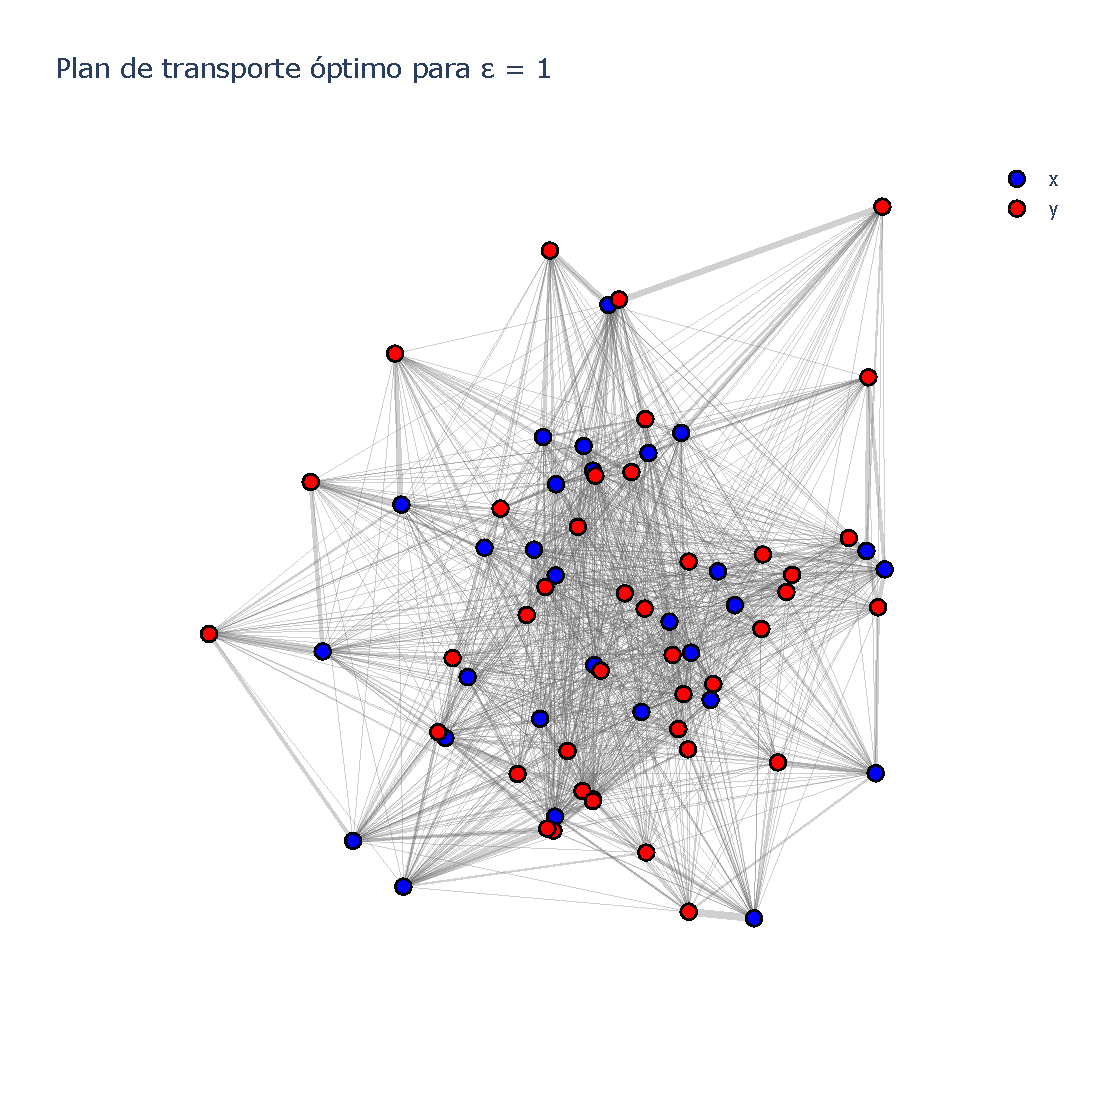
\includegraphics[width=0.45\textwidth]{images/eot_sbp/discrete_sinkhorn_graph1}
	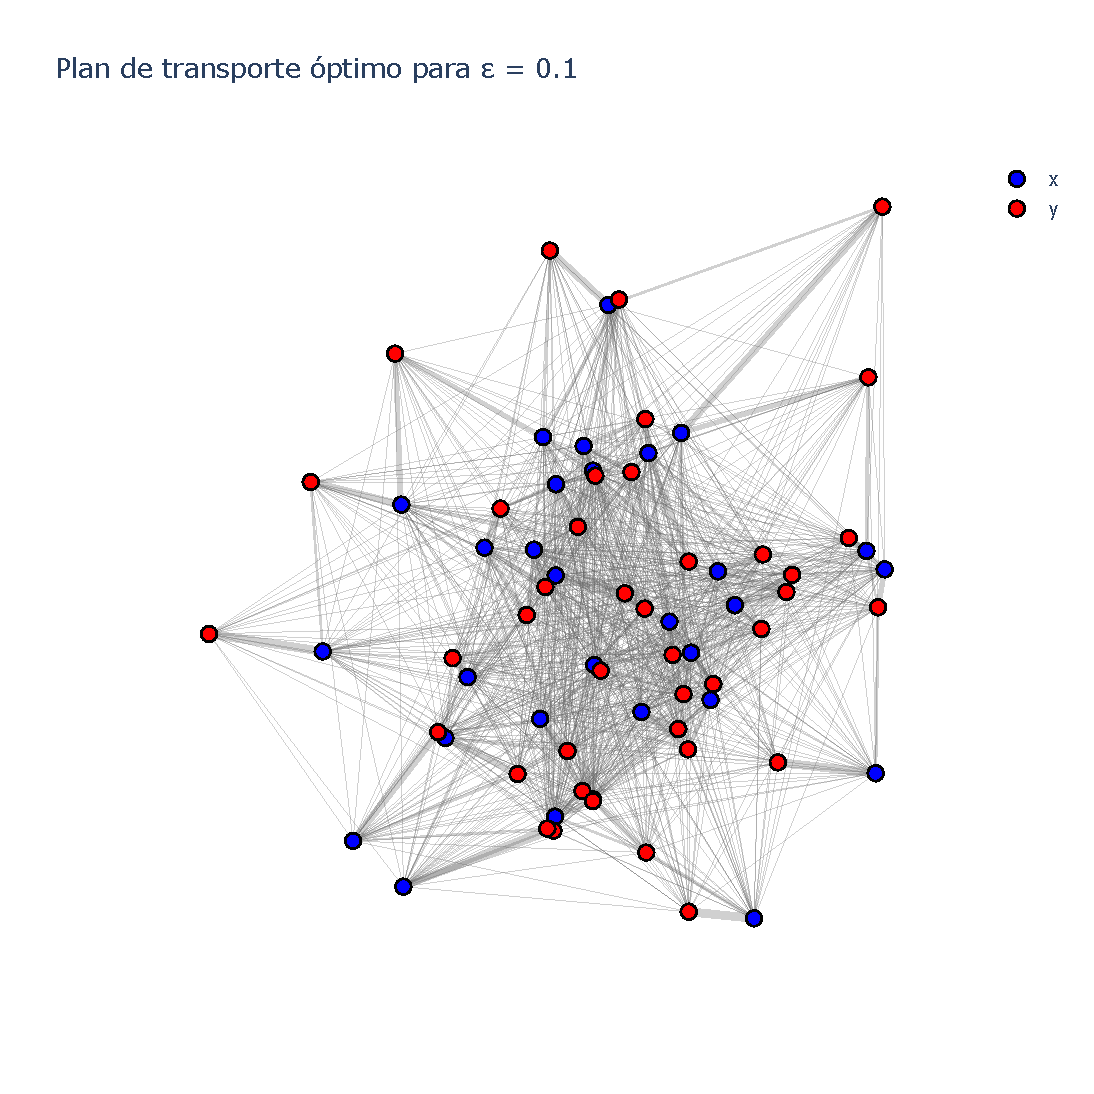
\includegraphics[width=0.45\textwidth]{images/eot_sbp/discrete_sinkhorn_graph0.1}
	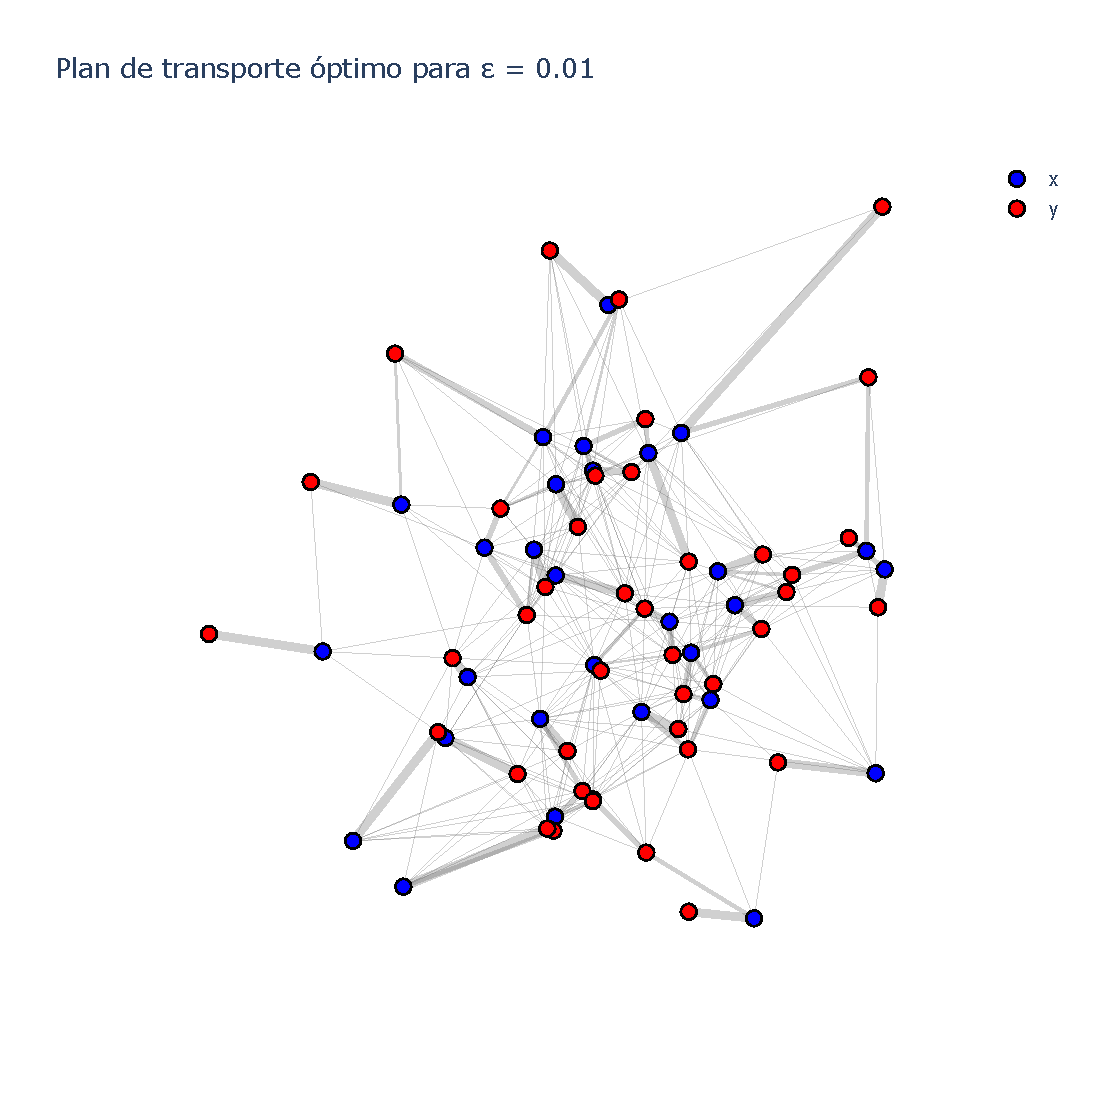
\includegraphics[width=0.45\textwidth]{images/eot_sbp/discrete_sinkhorn_graph0.01}
	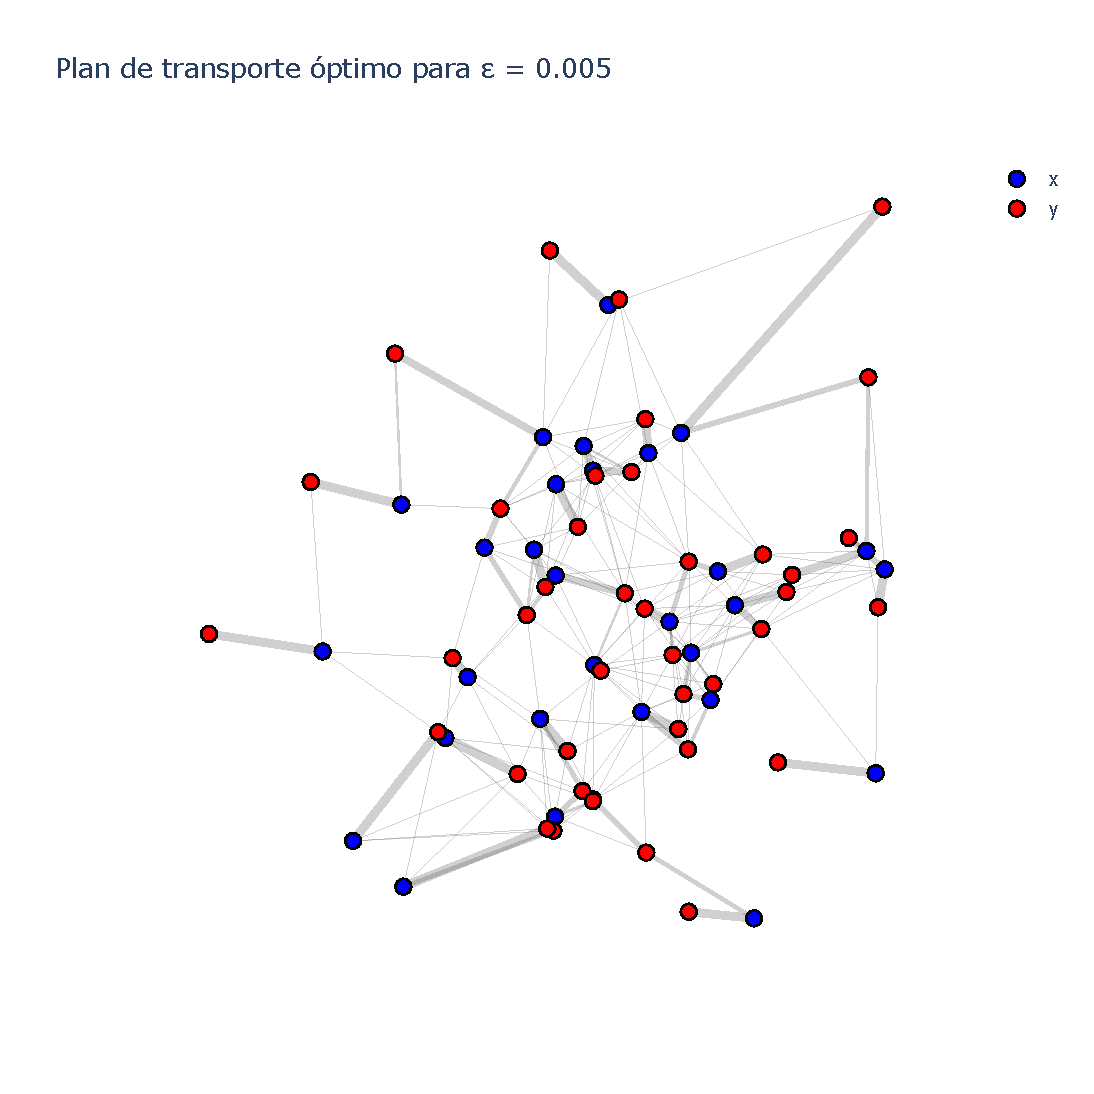
\includegraphics[width=0.45\textwidth]{images/eot_sbp/discrete_sinkhorn_graph0.005}
	\caption{Soluciones para el problema entrópico utilizando el \autoref{alg:sinkhorn}. El grusor de los arcos es proporcional a la cantidad de masa transferida según el plan de transporte. Se observa como el plan de transporte entrópico se va volviendo determinista a medida que disminuye $\epsilon$. Esta simulación se encuentra en el archivo \texttt{sinkhorn.ipynb}.}
	\label{fig:eot_sbp/discrete_sinkhorn_graph}
\end{figure}

Por último, es importante mencionar que las inicializaciones $v^{(0)} = \1_m$ y $P^{(0)}=\gibbs$ se puede sustituir por otras, pudiendo cambiando únicamente los valores finales de los vectores $u^{(l)}$ y $v^{(l)}$ pero no la convergencia de $P^{(l)} $a $P^*$. Además, este algoritmo se puede extender a su versión continua, donde el kernel de Gibbs toma la forma

\begin{equation*}
	\d\gibbs(x,y) = \exp\parent{-\frac{c(x,y)}{\epsilon}}\d\,\parent{\mu\otimes\nu}(x,y).
\end{equation*}

Esta extensión se puede revisar en \cite{nutz2022introduction}. Por otra parte, el \autoref{alg:sinkhorn} puede ser modificado para resolver el problema del baricentro de Wasserstein \eqref{eq:discrete_barycenter} cuando se aplica una regularización entrópica. En este caso, el problema del baricentro regularizado toma la forma

\begin{equation*}
	\argmin_{\feasible{a_B\in\Sigma_n}{(P_i)_{i=1}^k\subset \matrixspace{n,n}{[0,1]}}}
	\sum_{i=1}^k \lambda_i \KL{P_i}{\gibbs}
	\quad\text{sujeto a}\quad
	P_i\1_n = a_i,\, P_i^\top \1_n = a_B,\,\forall i\in\{1,\ldots,k\},
\end{equation*}

donde $\gibbs=\exp\parent{-\frac{\epsilon}{c}}$ es el kernel de Gibbs.


\subsubsection{Convergencia bajo la métrica de Hilbert}

En este apartado se estudiará la velocidad de convergencia del algoritmo de Sinkhorn a la solución óptima $P^*$ del problema entrópico discreto. Para esto, será necesario definir un espacio adecuado donde estudiar la noción de cercanía entre los elementos involucrados en el algoritmo de Sinkhorn. Dado que todas las soluciones del problema son de la forma $(ru^*, \frac{1}{r}v^*)$ con $r>0$ y $(u^*,v^*)$ una solución arbitraria, resulta útil la siguiente definición, la cual permite tratar a todos los vectores con la misma dirección como iguales:

\begin{defn}[cono proyectivo real]
	\label{defn:projective_cone}
	Dados dos vectores positivos $u,v\in\R^d_{++}$, se dirá que $u\sim v$ si existe un $r>0$ tal que $u=rv$. Con esto, se define el \textit{cono proyectivo real} como el espacio cociente inducido por esta relación de equivalencia:

	\begin{equation*}
		\cone{d}\, = \{[u]\,:\, u\in\R^d_{++}\},
	\end{equation*}

	donde $[u]=\{v\in\R_{++}^d:u\sim v\}$ es la clase de equivalencia de $u\in\R^d_{++}$, la cual representa el rayo con la dirección de $u$ en el ortante positivo.
\end{defn}

En este espacio, es usual definir la métrica proyectiva de Hilbert, la cual será usada para medir la cercanía entre las iteraciones del algoritmo de Sinkhorn, $\parent{u^{(l)}, v^{(l)}}$ y la solución $(u^*,v^*)$, la cual es única vista como un elemento de $\cone{d}$. Por simplicidad, se denotarán los elementos de $\cone{d}$ como vectores usuales en $\R_{++}^d$, teniendo siempre presente que solo importa la dirección de los vectores y no su magnitud.

\begin{prop}[métrica de Hilbert]
	Dados dos vectores $u,v\in\R^d_{++}$, se define la \textit{métrica proyectiva de Hilbert} como

	\begin{equation}
		\label{eq:hilbert_metric}
		\hmetric{u}{v} = \log\parent{\max_{1\leq i,j\leq d} \frac{u_i v_j}{v_i u_j}}.
	\end{equation}

	En $\cone{d}$, $\hmetric{\cdot}{\cdot}$ define una métrica y, más aún, esta métrica es completa\footnote{Si bien esta es una propiedad técnica, es esencial para usar resultados como el teorema del punto fijo de Banach, el cual permite concluir la convergencia del algoritmo de Sinkhorn.}.

\end{prop}

Notar que $\hmetric{\cdot}{\cdot}$ está bien definida para elementos de $\cone{d}$. En efecto, si $p\in[u]$ y $q\in[v]$ (i.e., existen $r,s>0$ tales que $p=ru$ y $q=sv$), entonces:

\begin{equation*}
	\hmetric{p}{q}
	= \log\parent{\max_{1\leq i,j\leq d} \frac{(ru_i)(sv_j)}{(sv_i)(ru_j)}}
	= \log\parent{\max_{1\leq i,j\leq d} \frac{u_i v_j}{v_i u_j}}
	= \hmetric{u}{v}.
\end{equation*}

Por lo que la distancia no depende del representante de $[u]$ o $[v]$. En la \autoref{fig:eot_sbp/hilbert_metric} se puede observar la distancia entre dos elementos del cono proyectivo $\cone{2}$.

\insertimage{eot_sbp/hilbert_metric}{0.3}{Distancia de Hilbert entre dos rayos $u,u'\in\cone{}$, donde la distancia depende únicamente del ángulo entre ambos rayos. Imagen obtenida desde \cite{peyré2020computational}.}

El siguiente resultado afirma que si $M$ es una matriz de entradas positivas, la distancia entre los rayos $Mu$ y $Mv$ es menor que la distancia entre los rayos $u$ y $v$. Es decir, al multiplicar rayos por matrices positivas, estos se vuelven cada vez más cercanos. Esto puede verse en la \autoref{fig:eot_sbp/hilbert_contraction}.

\begin{teo}[contracciones en $\cone{d}$]
	Dada una matriz con entradas positivas, $M\in\matrixspace{n,m}{\R_{++}}$, entonces el operador $x\in\cone{d} \mapsto \ Mx\in\cone{d}$ es una contracción, es decir:

	\begin{equation*}
		\hmetric{Mu}{Mv} \leq \lambda(M)\, \hmetric{u}{v}
		\quad \forall u,v\in\cone{d},
	\end{equation*}

	donde $\lambda(M)<1$ es una constante que depende únicamente de $M$.

\end{teo}

\insertimage{eot_sbp/hilbert_contraction}{0.8}{Contracción del primer cuadrante en $\R^2$ provocada por la multiplicación consecutiva de una matriz positiva $K$. Se observa que a medida que se va multiplicando por $K$, los rayos están cada vez más cerca, convergiendo a un único rayo en el cuadrante positivo. Imagen obtenida desde \cite{peyré2020computational}.}

Este resultado permite mostrar que las iteraciones $(u^{(l)},v^{(l)})$ se van acercando cada vez más a la solución real $(u^*,v^*)$, la cual es única salvo ponderaciones positivas (i.e., es única vista como elemento de $\cone{n}$ y $\cone{m}$ respectivamente). En efecto, de \eqref{eq:sinkhorn_u_update} se tiene que:

\begin{equation*}
	u^{(l+1)} = a \oslash \parent{\gibbs v^{(l)}}
	\quad\text{y}\quad
	u^* = a \oslash \parent{\gibbs v^*}.
\end{equation*}

Luego, notando que la distancia en \eqref{eq:hilbert_metric} no cambia si las coordenadas de $u$ y $v$ se ponderan por un mismo vector, se tiene lo siguiente:

\begin{align*}
	\hmetric{u^{(l+1)}}{u^*} &= \hmetric{a \oslash \parent{\gibbs v^{(l)}}}{a \oslash \parent{\gibbs v^*}}\\
	&= \hmetric{\1_n \oslash \parent{\gibbs v^{(l)}}}{1_n \oslash \parent{\gibbs v^*}}\\
	&= \hmetric{\parent{\gibbs v^*} \oslash \parent{\gibbs v^{(l)}}}{\1_n}\\
	&= \hmetric{\gibbs v^*}{\gibbs v^{(l)}}\\
	&\leq \lambda(\gibbs)\, \hmetric{v^*}{v^{(l)}}.
\end{align*}

Del mismo modo, de \eqref{eq:sinkhorn_v_update} se obtiene que $\hmetric{v^{(l+1)}}{v^*} \leq \lambda(\gibbs)\, \hmetric{u^*}{u^{(l+1)}}$. Por lo tanto, sustituyendo esta expresión y por inducción se concluye que:

\begin{equation*}
	\hmetric{u^{(l)}}{u^*}
	\leq \lambda(\gibbs)^2\, \hmetric{u^{(l-1)}}{u^*}
	\leq \lambda(\gibbs)^{2l}\, \hmetric{u^{(0)}}{u^*}.
\end{equation*}

De forma análoga se demuestra que $\hmetric{v^{(l)}}{v^*} \leq \lambda(\gibbs)^{2l}\, \hmetric{v^{(0)}}{v^*}$.

Por otra parte, estas desigualdades permiten acotar la distancia a las soluciones óptimas $u^*$ y $v^*$ mediante la discrepancia entre las distibuciones marginales de $P^{(l)}$ y las marginales esperadas $\mu$ y $\nu$. En efecto, usando la desigualdad triangular:

\begin{equation*}
	\hmetric{u^{(l)}}{u^*}
	\leq \hmetric{u^{(l)}}{u^{(l+1)}} + \hmetric{u^{(l+1)}}{u^*}
	\leq \hmetric{u^{(l)}}{a\oslash \parent{Kv^{(l)}}} + \lambda(\gibbs)^2\, \hmetric{u^{(l)}}{u^*}.
\end{equation*}

Por lo tanto:

\begin{equation*}
	\hmetric{u^{(l)}}{u^*}
	\leq \frac{\hmetric{u^{(l)}}{a\oslash \parent{Kv^{(l)}}}}{1-\lambda(\gibbs)^2}
	= \frac{\hmetric{u^{(l)}\odot \parent{Kv^{(l)}}}{a}}{1-\lambda(\gibbs)^2}
	= \frac{\hmetric{P^{(l)}\1_m}{a}}{1-\lambda(\gibbs)^2}.
\end{equation*}

Mientras que para la segunda marginal se demuestra de forma equivalente que

\begin{equation*}
	\hmetric{v^{(l)}}{v^*}
	\leq \frac{\hmetric{\parent{P^{(l)}}^\top\1_n}{b}}{1-\lambda(\gibbs)^2}.
\end{equation*}


Estas propiedades se resumen en el siguiente teorema, el cual, además, incluye una cota para la distancia uniforme entre $P^*$ y $P^{(l)}$:

\begin{teo}[convergencia del algoritmo de Sinkhorn]
	\label{teo:sinkhorn_convergence}
	Dadas las iteraciones \eqref{eq:sinkhorn_u_update} y \eqref{eq:sinkhorn_v_update} del algoritmo de Sinkhorn, entonces:

	\begin{equation*}
		\parent{u^{(l)},v^{(l)}} \to \parent{u^*,v^*}
		\quad\text{en }\cone{d}.
	\end{equation*}

	Además, si $P^*$ es la (única) solución del problema entrópico \eqref{eq:eot_discrete_kl} y $P^{(l)} = \diag{u^{(l)}}\gibbs\diag{v^{(l)}}$ es su aproximación dada por el \autoref{alg:sinkhorn}, entonces:

	\begin{equation}
		\label{eq:sinkhorn_p_bound}
		\norm{\log P^{(l)} - \log P^*}_\infty \leq \hmetric{u^{(l)}}{u^*} + \hmetric{v^{(l)}}{v^*},
	\end{equation}

	donde

	\begin{equation}
		\label{eq:sinkhorn_uv_bound}
		\hmetric{u^{(l)}}{u^*}\leq\frac{\hmetric{P^{(l)}\1_m}{a}}{1-\lambda(\gibbs)^2}
		\quad\text{y}\quad
		\hmetric{v^{(l)}}{v^*}\leq \frac{\hmetric{\parent{P^{(l)}}^\top\1_n}{b}}{1-\lambda(\gibbs)^2},
	\end{equation}

	más aún, estas distancias decaen de forma exponencial:

	\begin{equation*}
		\hmetric{u^{(l)}}{u^*} = \mathcal{O}(\lambda(\gibbs)^{2l})
		\quad\text{y}\quad
		\hmetric{v^{(l)}}{v^*} = \mathcal{O}(\lambda(\gibbs)^{2l}).
	\end{equation*}

\end{teo}

El resultado anterior muestra una convergencia lineal para el algoritmo de Sinkhorn. Además, las desigualdades \eqref{eq:sinkhorn_p_bound} y \eqref{eq:sinkhorn_uv_bound} indican que las discrepancias entre las marginales de $P^{(l)}$ y los vectores de probabilidad $a\in\Sigma_n$ y $b\in\Sigma_m$ son un buen criterio de parada para este algoritmo. Esto puede observarse en la \autoref{fig:eot_sbp/discrete_sinkhorn_matrix} para el caso discreto y en la \autoref{fig:eot_sbp/discrete_sinkhorn_matrix1} para el caso continuo, donde además se grafica la proyección baricéntrica del plan de transporte entrópico, la cual permite obtener, de manera forzada, un mapa $T:\xspace\to\yspace$ mediante el promedio en $\yspace$ del plan de Kantorovich $\pi$:

\begin{equation*}
	T(x) = \int_\yspace y \frac{\d\pi}{\d,(\mu\otimes\nu)}(x,y) \d\nu(y).
\end{equation*}

\begin{figure}[!ht]
	\centering
	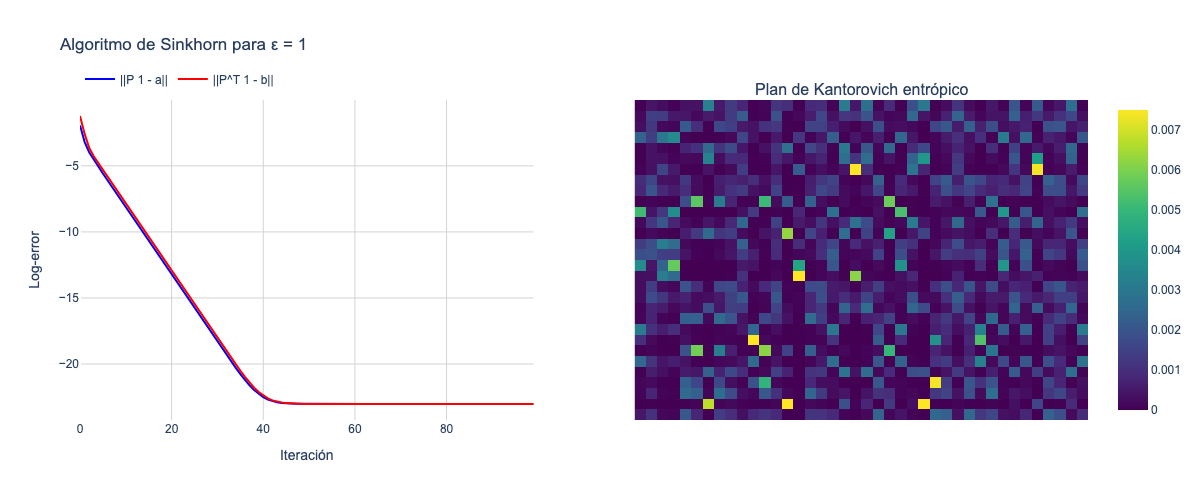
\includegraphics[width=0.75\textwidth]{images/eot_sbp/discrete_sinkhorn_matrix1}
	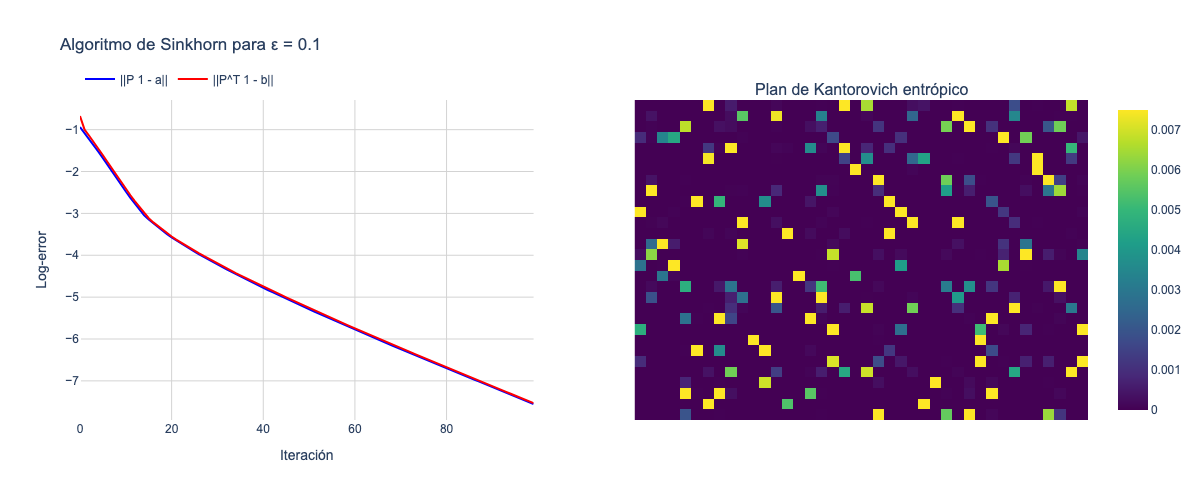
\includegraphics[width=0.75\textwidth]{images/eot_sbp/discrete_sinkhorn_matrix0.1}
	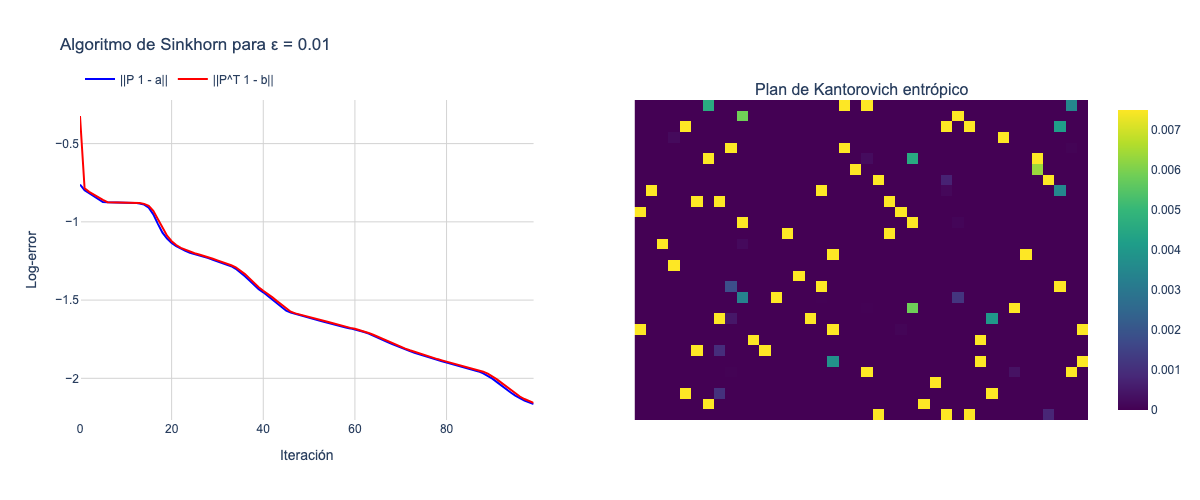
\includegraphics[width=0.75\textwidth]{images/eot_sbp/discrete_sinkhorn_matrix0.01}
	\caption{Iteraciones del algoritmo de Sinkhorn entre dos distribuciones discretas Se observa que a medida se disminuye $\epsilon$, el error disminuye más lentamente, mientras que el plan de transporte se vuelve más determinista. La simulación se encuentra en el archivo \texttt{sinkhorn.ipynb}.}
	\label{fig:eot_sbp/discrete_sinkhorn_matrix}
\end{figure}

\begin{figure}[!ht]
	\centering
	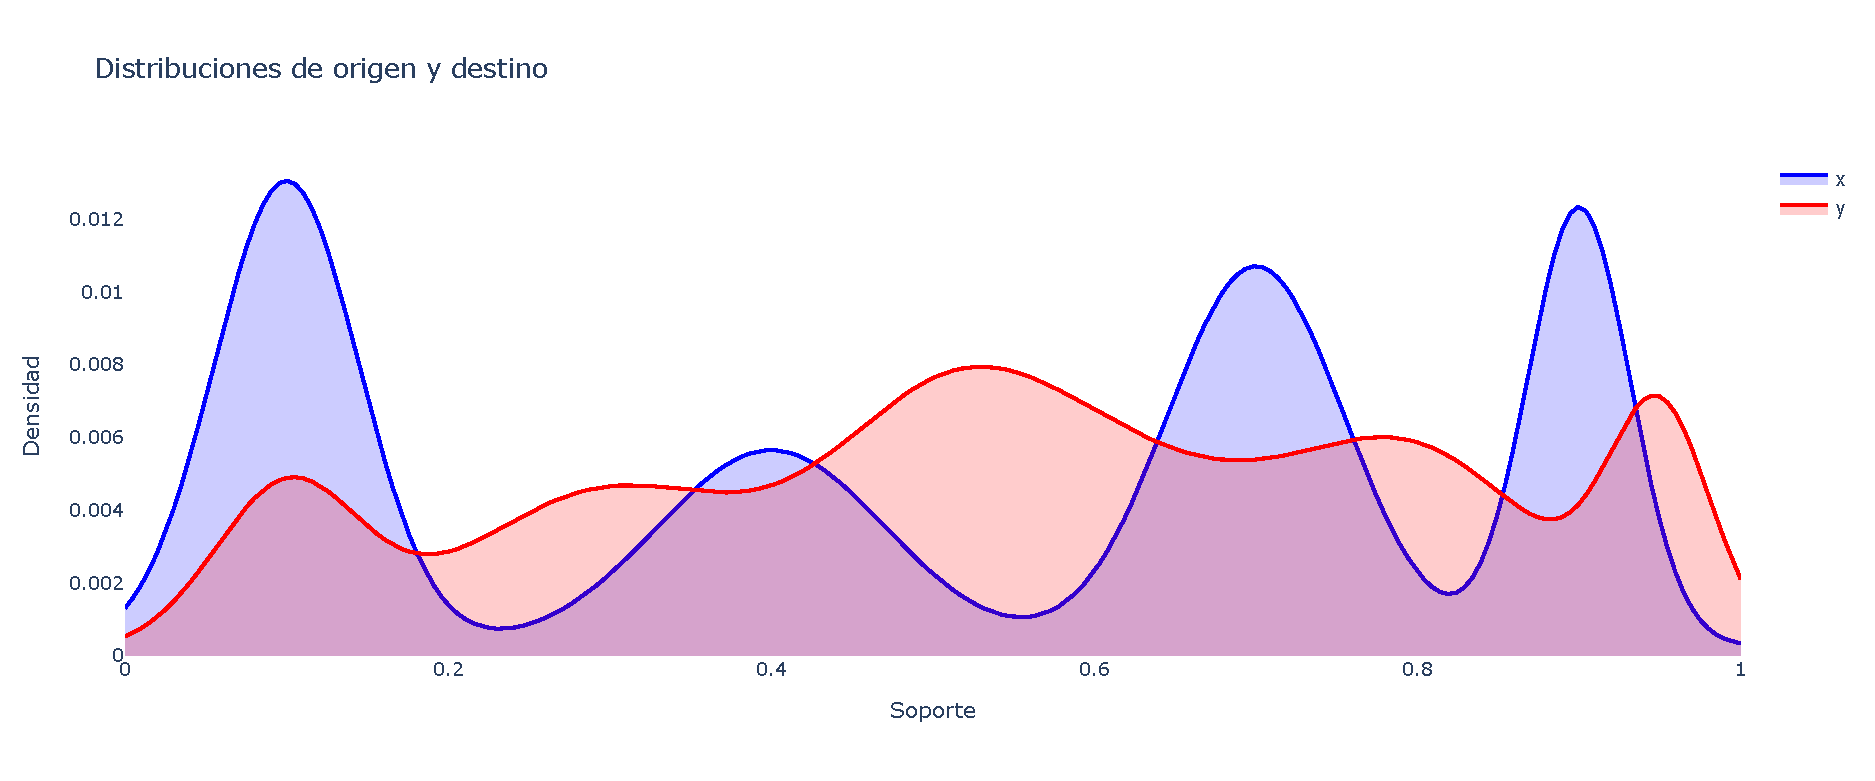
\includegraphics[width=0.7\textwidth]{images/eot_sbp/continuous_sinkhorn_density}
	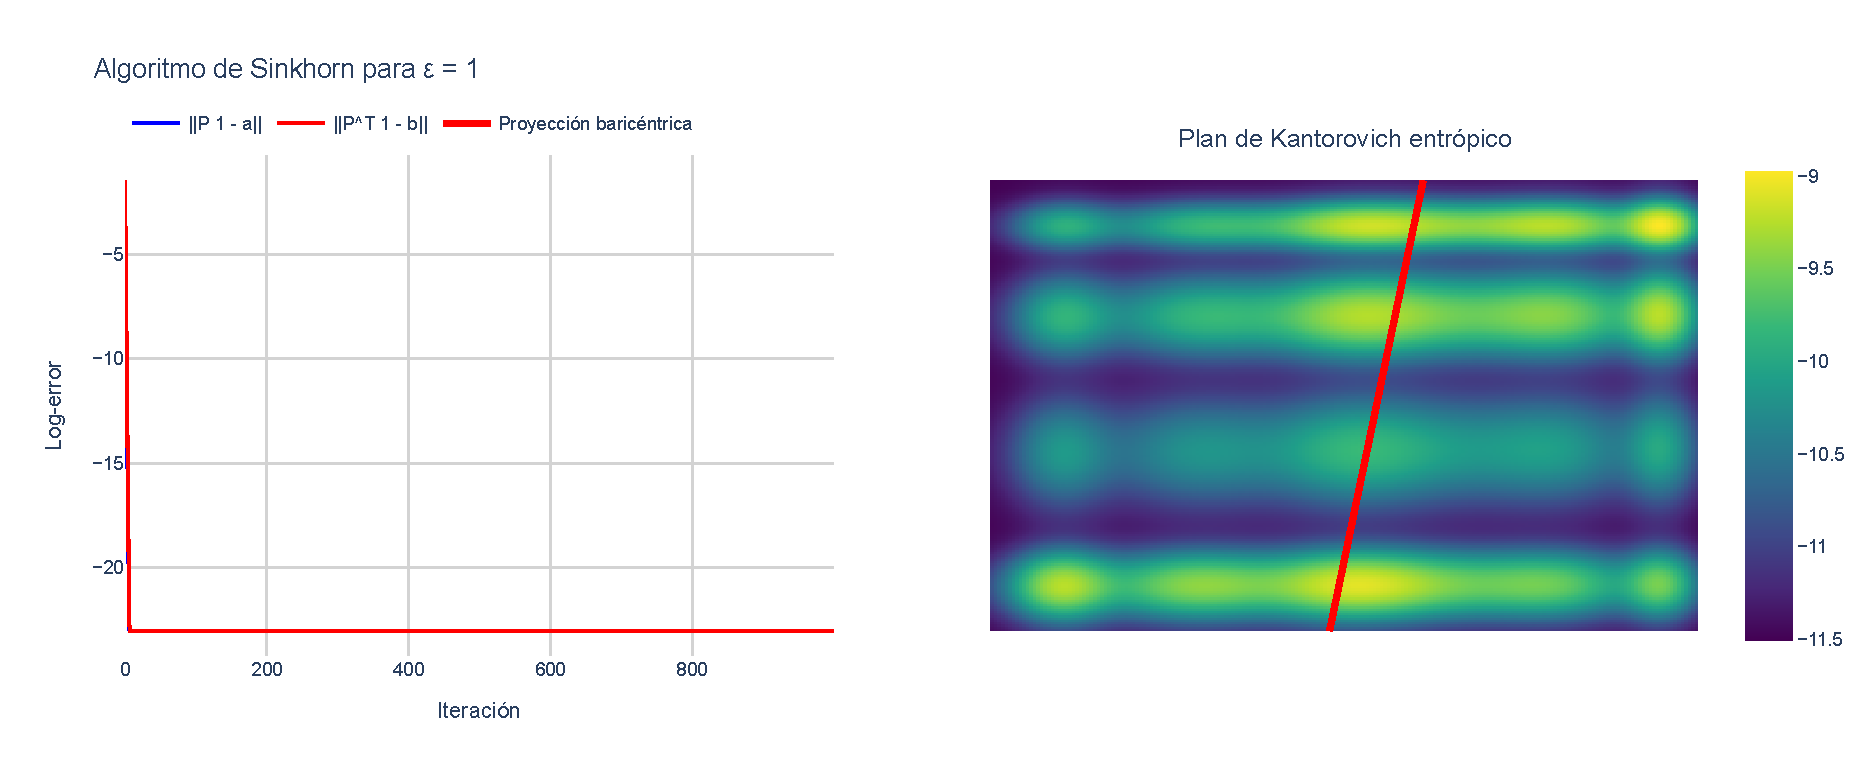
\includegraphics[width=0.7\textwidth]{images/eot_sbp/continuous_sinkhorn_matrix1}
	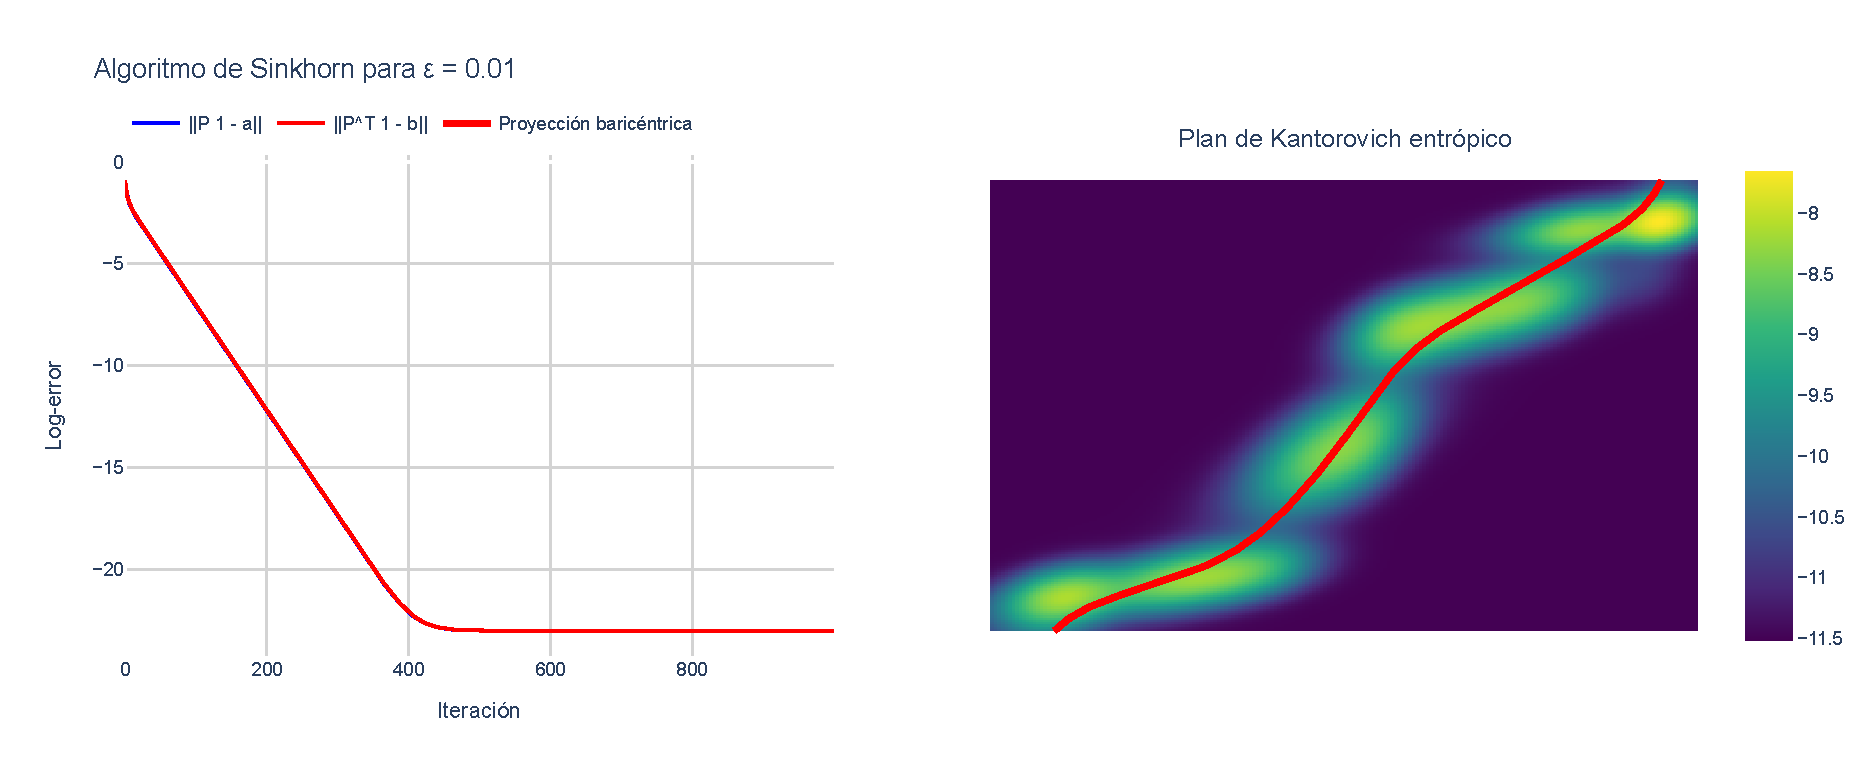
\includegraphics[width=0.7\textwidth]{images/eot_sbp/continuous_sinkhorn_matrix0.01}
	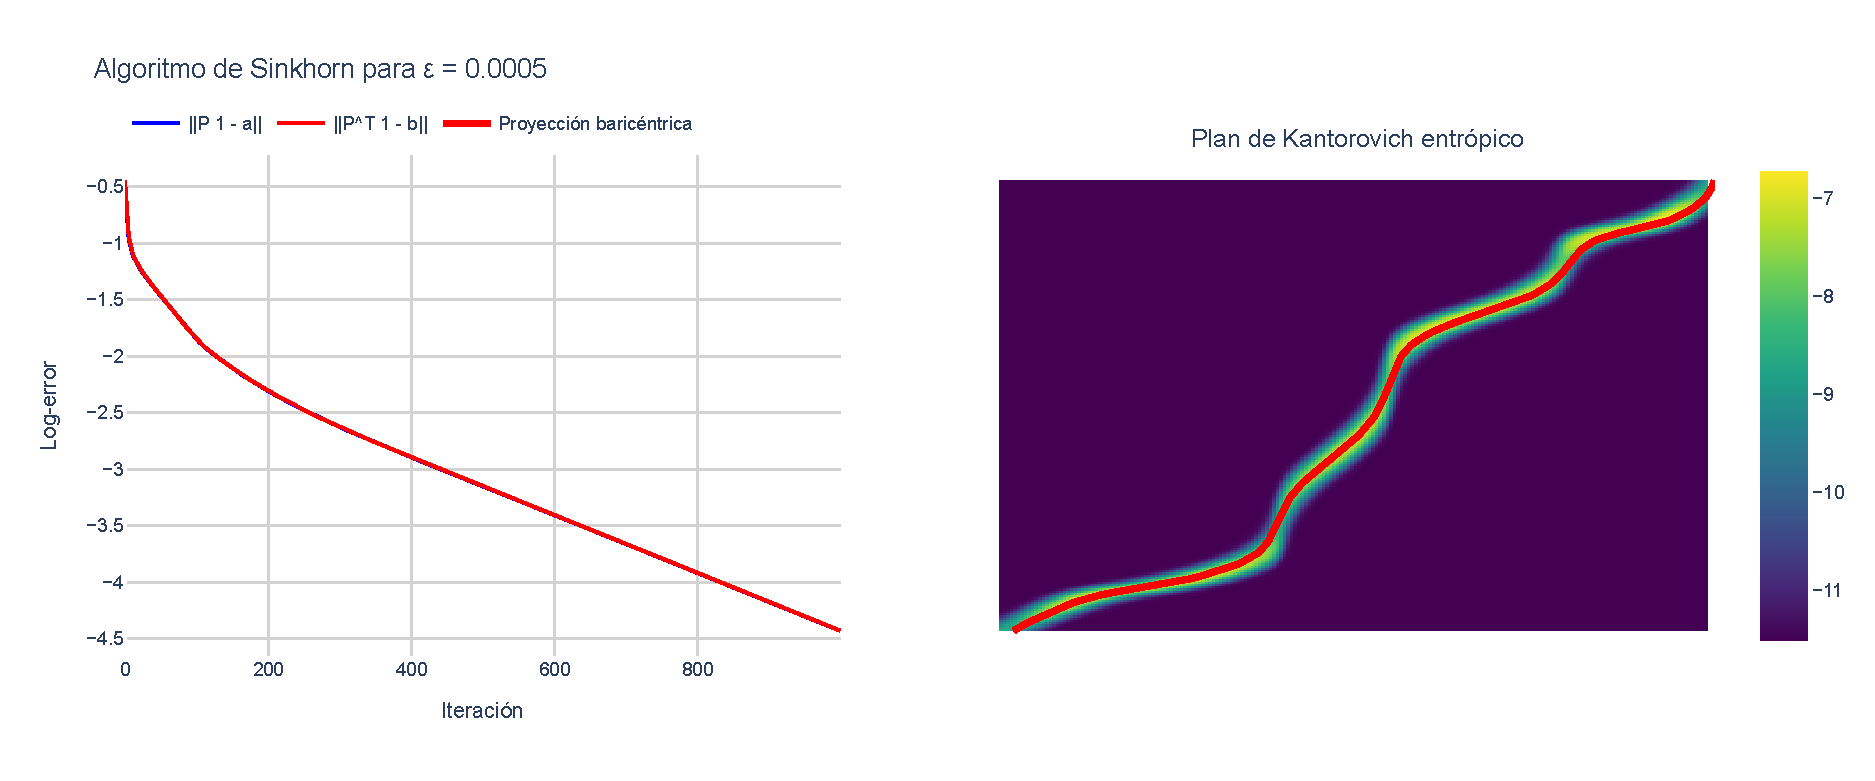
\includegraphics[width=0.7\textwidth]{images/eot_sbp/continuous_sinkhorn_matrix0.0005}
	\caption{Iteraciones del algoritmo de Sinkhorn entre dos distribuciones continuas. Se observa que la proyección baricéntrica del plan de transporte óptimo converge al mapa de Monge del problema cuando $\epsilon\to0$. Además, se observa que para $\epsilon=1$ la solución (similar a la medida producto) se encuentra en muy pocas iteraciones. La simulación se encuentra en el archivo \texttt{sinkhorn.ipynb}.}
	\label{fig:eot_sbp/discrete_sinkhorn_matrix1}
\end{figure}

\section{Formulación dinámica}
\label{eot_sbp/dynamic}

De forma similar a lo realizado para el problema de Kantorovich no regularizado, es posible formular el problema de Schrödinger \eqref{eq:static_sbp} como un problema dinámico. En esta marco de trabajo, el objetivo es encontrar un proceso estocástico $x=(x_t)_{t\in[0,1]}$ que tenga ciertas distribuciones marginales al comienzo y al final del proceso, y que además esté lo más cerca posible (en el sentido de la entropía relativa) a un proceso estocástico de referencia:

\begin{defn}[problema del puente de Schrödinger, versión dinámica]
	Considerando $\xspace=\yspace\subset\R^d$, el puente de Schrödinger entre las medidas $\mu\in\probmeasure{\xspace}$ y $\nu\in\probmeasure{\yspace}$ dada una medida de referencia $R\in\probmeasure{C([0,1],\xspace)}$ es la (única) solución del problema

	\begin{equation}
		\label{eq:dynamic_sbp}
		\argmin_{P\in\Gamma(\mu,\nu)} \KL{P}{R},
	\end{equation}
\end{defn}

donde, al igual que en el \autoref{dm}, $\Gamma(\mu,\nu)$ el conjunto de medidas de probabilidad en $C^1([0,1],\xspace)$ cuyas marginales en $t=0$ y $t=1$ son $\mu$ y $\nu$ respectivamente:

\begin{equation*}
	\Gamma(\mu,\nu) = \{P\in \probmeasure{C([0,1],\xspace)}: P_0=\mu, P_1 = \nu\}.
\end{equation*}

Sorprendentemente, este problema puede ser resuelto fácilmente si se conoce una solución para el problema de Schrödinger estático \eqref{eq:static_sbp}. En efecto, la divergencia $\KL{P}{R}$ entre dos procesos estocásticos se puede descomponer en la divergencia entre su marginales en tiempo $t\in\{0,1\}$ y el resto del proceso en tiempo $t\in(0,1)$. Para ver esto, se tiene la siguiente descomposición de la entropía relativa cuando está definida sobre medidas en un espacio producto:

\begin{prop}[regla de la cadena para la entropía relativa]
	Sean $\mu,\nu\in\probmeasure{\xspace\times\yspace}$ dos medidas de probabilidad definidas en un espacio producto, entonces:

	\begin{equation*}
		\KL{\mu}{\nu} = \KL{\mu_0}{\nu_0} + \E{x\sim\mu_0}{\KL{\mu_{|x}}{\nu_{|x}}},
	\end{equation*}

	donde $\mu_0$ y $\nu_0$ son la primera marginal de $\mu$ y $\nu$ respectivamente, mientras que $\mu_{|x}$ y $\nu_{|x}$ corresponden a la segunda marginal condicionada a que la primera componente sea $x$.
\end{prop}

\begin{proof}
	Por simplicidad en la notación, se asumirá que $\mu$ y $\nu$ poseen función de densidad $p_\nu(x,y)$ y $p_\nu(x,y)$ respectivamente. De esta forma:

	\begin{align*}
		\KL{\mu}{\nu} &= \int_{\xspace\times\yspace} \log\parent{\frac{p_\mu(x,y)}{p_\nu(x,y)}} p_\mu(x,y) \d\,(x,y)\\
		&= \int_{\xspace\times\yspace} \log\parent{\frac{p_\mu(x)}{p_\nu(x)}} p_\mu(x)p_\mu(y|x) \d\,(x,y) + \int_{\xspace\times\yspace} \log\parent{\frac{p_\mu(y|x)}{p_\nu(y|x)}} p_\mu(x)p_\mu(y|x) \d\,(x,y)\\
		&= \int_{\xspace} \log\parent{\frac{p_\mu(x)}{p_\nu(x)}} p_\mu(x)\parent{\int_\yspace p_\mu(y|x) \d y}\d x + \int_{\xspace} \rparent{\log\parent{\frac{p_\mu(y|x)}{p_\nu(y|x)}} p_\mu(y|x) \d y}p_\mu(x) \d x\\
		&= \KL{p_\mu(x)}{p_\nu(x)} + \E{x\sim p_\mu(x)}{\KL{p_\mu(y|x)}{p_\nu(y|x)}}.
	\end{align*}
\end{proof}

En consecuencia, $\KL{P}{R}$ admite la siguiente descomposición:

\begin{equation*}
	\KL{P}{R} = \KL{P_{01}}{R_{01}} + \E{(x,y)\sim P_{01}}{\KL{P_{|xy}}{R_{|xy}}},
\end{equation*}

donde $P_{01},R_{01}\in\probmeasure{\xspace\times\yspace}$ son las medidas marginales de los procesos en tiempo $t=0$ y $t=1$, mientras que $P_{|xy}, R_{|xy}$ indican las medidas de los procesos condicionados a empezar en $x$ y terminar en $y$.

Por otra parte, notar que para el problema dinámico \eqref{eq:dynamic_sbp} se puede elegir $P_{|xy}=R_{|xy}$ para hacer el segundo sumando nulo. De esta forma:

\begin{equation*}
	\min_{P\in\Gamma(\mu,\nu)} \KL{P}{R} = \min_{P_{01}\in\Pi(\mu,\nu)} \KL{P_{01}}{R_{01}}.
\end{equation*}

Es decir, el problema dinámico tiene el mismo valor óptimo que el problema estático. Más aún, si $P_{01}^*$ resuelve el problema estático, entonces la medida

\begin{equation*}
	P^*(\cdot) = \int_{\xspace\times\yspace} R_{|xy}(\cdot) \d P_{01}^*(x,y),
\end{equation*}

resuelve el problema dinámico, mostrando que ambos problemas son equivalentes.

Por otro lado, cuando se considera como proceso de referencia a un movimiento browniano de difusividad $\epsilon$ (ver \autoref{defn:brownian_motion}), el problema de Schrödinger se reduce al problema de transporte óptimo entrópico con costo cuadrático

\begin{prop}[SBP browniano estático]
	Dado $P\in\Gamma(\mu,\nu)$ y $W^\epsilon$ un movimiento browiano con difusividad $\epsilon$, entonces:

	\begin{equation*}
		\KL{P_{01}}{W_{01}^\epsilon} = 
		\frac{1}{\epsilon}\rparent{\int_{\xspace\times\yspace} \frac{1}{2} \norm{x-y}^2 \d P_{01}(x,y) - \epsilon\cdot\entropy{P_{01}} + \cte}.
	\end{equation*}

\end{prop}

\begin{proof}
	Dado que $W^\epsilon$ es un movimiento browniano de difusividad $\epsilon$, $\frac{\d W_{1|0}^\epsilon}{\d y}(y|x)$ es la función de densidad de una variable aleatoria gaussiana, por lo que resulta conveniente realizar la siguiente descomposición:

	\begin{equation*}
		\frac{\d W_{01}^\epsilon}{\d x\d y}(x,y) = \frac{\d W_{1|0}^\epsilon}{\d y}(y|x) \cdot \underbrace{\frac{\d W_{0}^\epsilon}{\d x}(x)}_{\frac{\d\mu}{\d x}(x)},
		\qquad
		\d P_{01}(x,y) = \d P_{1|0}(y|x) \underbrace{\d P_0(x)}_{\d\mu(x)}.
	\end{equation*}

	Con esto:

	\begin{align*}
		\KL{P_{01}}{W_{01}^\epsilon} &= \int_{\xspace\times\yspace} \log\parent{\frac{\d P_{01}}{\d W_{01}^\epsilon}} \d P_{01}(x,y)\\
		&= \int_{\xspace\times\yspace} \log\parent{\frac{\d P_{01}}{\d x\d y}} \d P_{01}(x,y) - \int_{\xspace\times\yspace} \log\parent{\frac{\d W_{01}^\epsilon}{\d x\d y}} \d P_{01}(x,y)\\
		&= - \entropy{P_{01}} - \int_{\xspace\times\yspace} \log\rparent{\frac{1}{(2\pi\epsilon)^{\frac{d}{2}}} \exp\parent{\frac{-1}{2\epsilon} \norm{x-y}^2 } \cdot\frac{\d\mu}{\d x}(x)} \d P_{01}(x,y)\\
		&= - \entropy{P_{01}} + \frac{d}{2}\log(2\pi\epsilon) + \int_{\xspace\times\yspace} \frac{1}{2\epsilon} \norm{x-y}^2 \d P_{01}(x,y) - \int_{\xspace\times\yspace} \log\parent{\frac{\d\mu}{\d x}(x)} \d P_{01}(x,y)\\
		&= \int_{\xspace\times\yspace} \frac{1}{2\epsilon} \norm{x-y}^2 \d P_{01}(x,y) - \entropy{P_{01}} - \underbrace{\int_\xspace \log\parent{\frac{\d\mu}{\d x}(x)} \parent{\int_\yspace \d P_{1|0}(y|x)} \d\mu(x)}_{-\entropy{\mu}} + \cte\\
		&= \frac{1}{\epsilon}\rparent{\int_{\xspace\times\yspace} \frac{1}{2} \norm{x-y}^2 \d P_{01}(x,y) - \epsilon\cdot\entropy{P_{01}} + \cte}.
		\end{align*}

\end{proof}

A modo de ejemplo, en la \autoref{fig:sbp} se muestran algunos puentes de Schrödinger trazados entre dos distribuciones discretas. Es importante destacar que lo único necesario para realizar esto es resolver el problema entrópico con costo cuadrático, ya que la distribución condicional $W_{|xy}$ del movimiento browiano empezando en $x$ y terminando en $y$ es totalmente conocida y se denomina \textit{puente browniano}, el cual tiene la siguiente SDE:

\begin{equation*}
	\d x_t = \frac{y-x_t}{1-t} \d t + \d w_t
\end{equation*}

donde se consideró, por simplicidad, que la difusión es constante y unitaria. En la \autoref{fig:eot_sbp/brownian_bridge} se puede ver un puente browiano unidimensional.

\insertimage{eot_sbp/brownian_bridge}{0.7}{Puente browniano entre los puntos $x_0=2$ y $x_1=5$. Esta simulación se encuentra en el archivo \texttt{sdes.ipynb}.}

\begin{figure}[!ht]
	\centering
	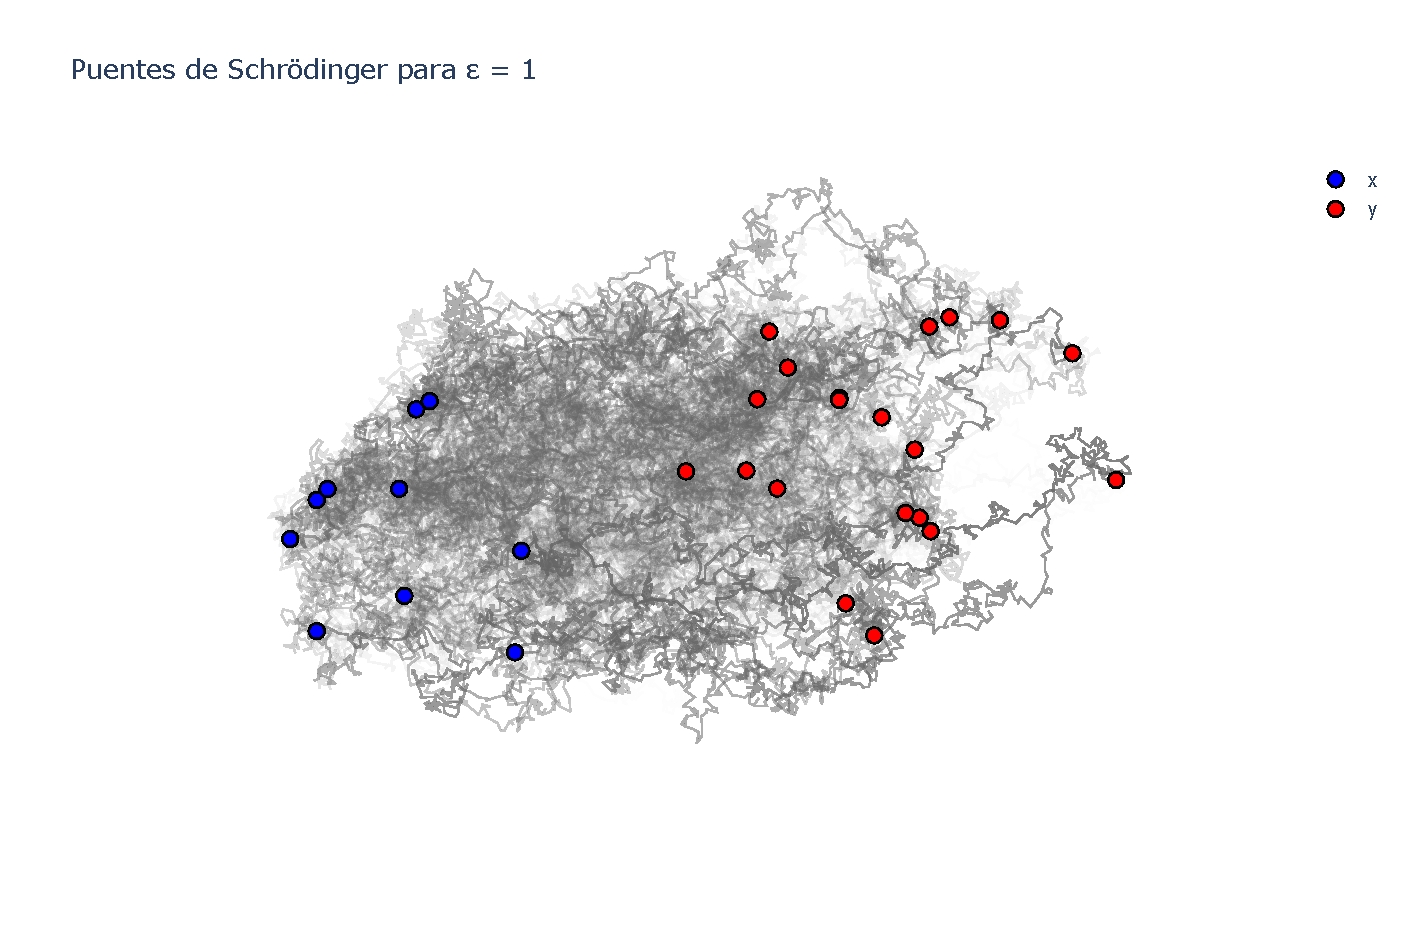
\includegraphics[width=0.7\textwidth]{images/eot_sbp/sbp_solution1}
	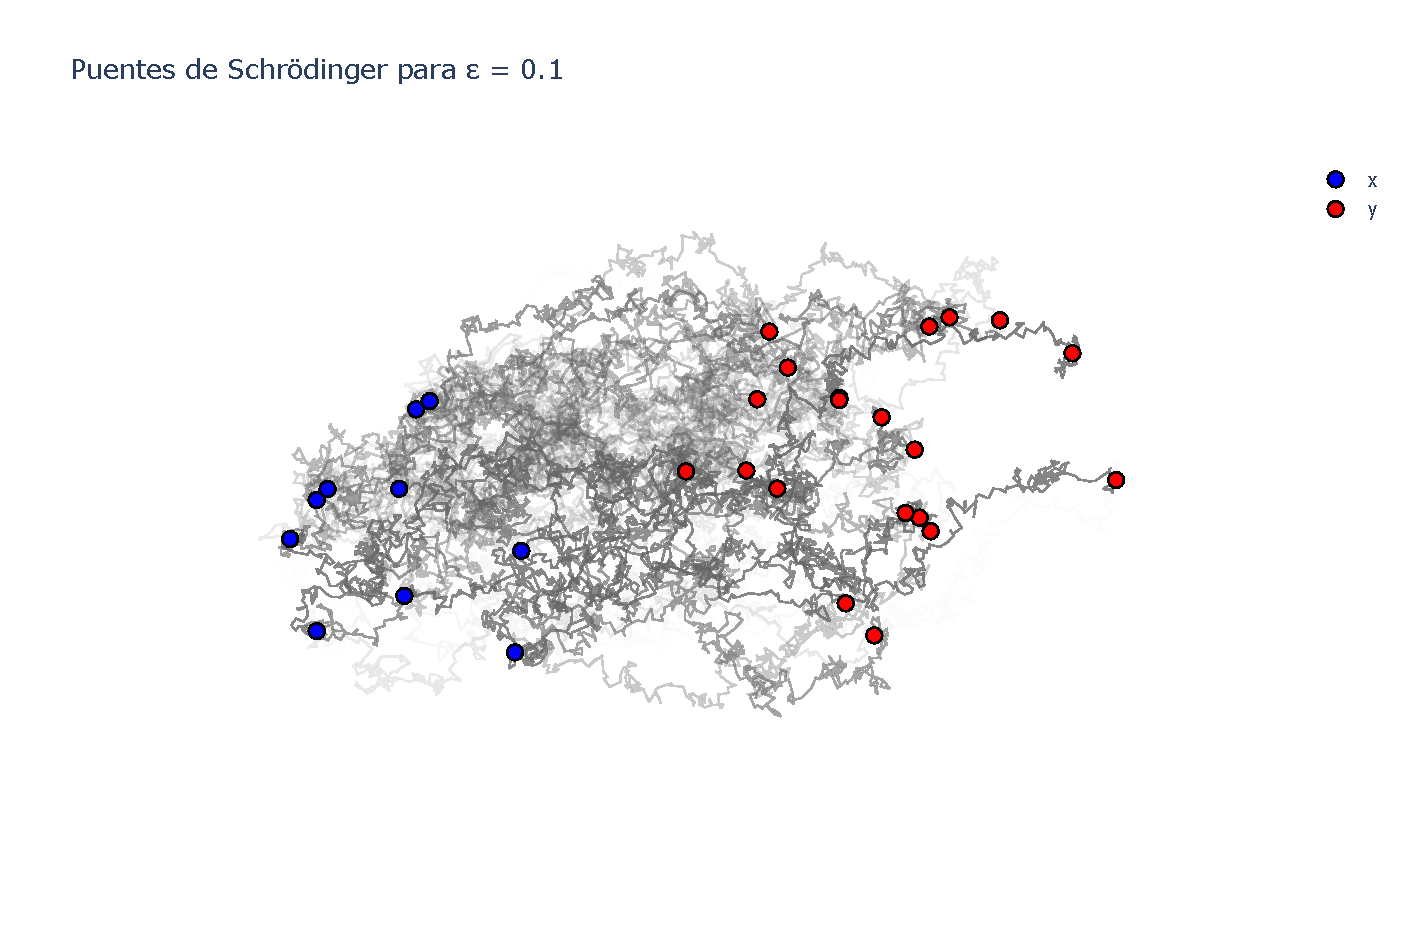
\includegraphics[width=0.7\textwidth]{images/eot_sbp/sbp_solution0.1}
	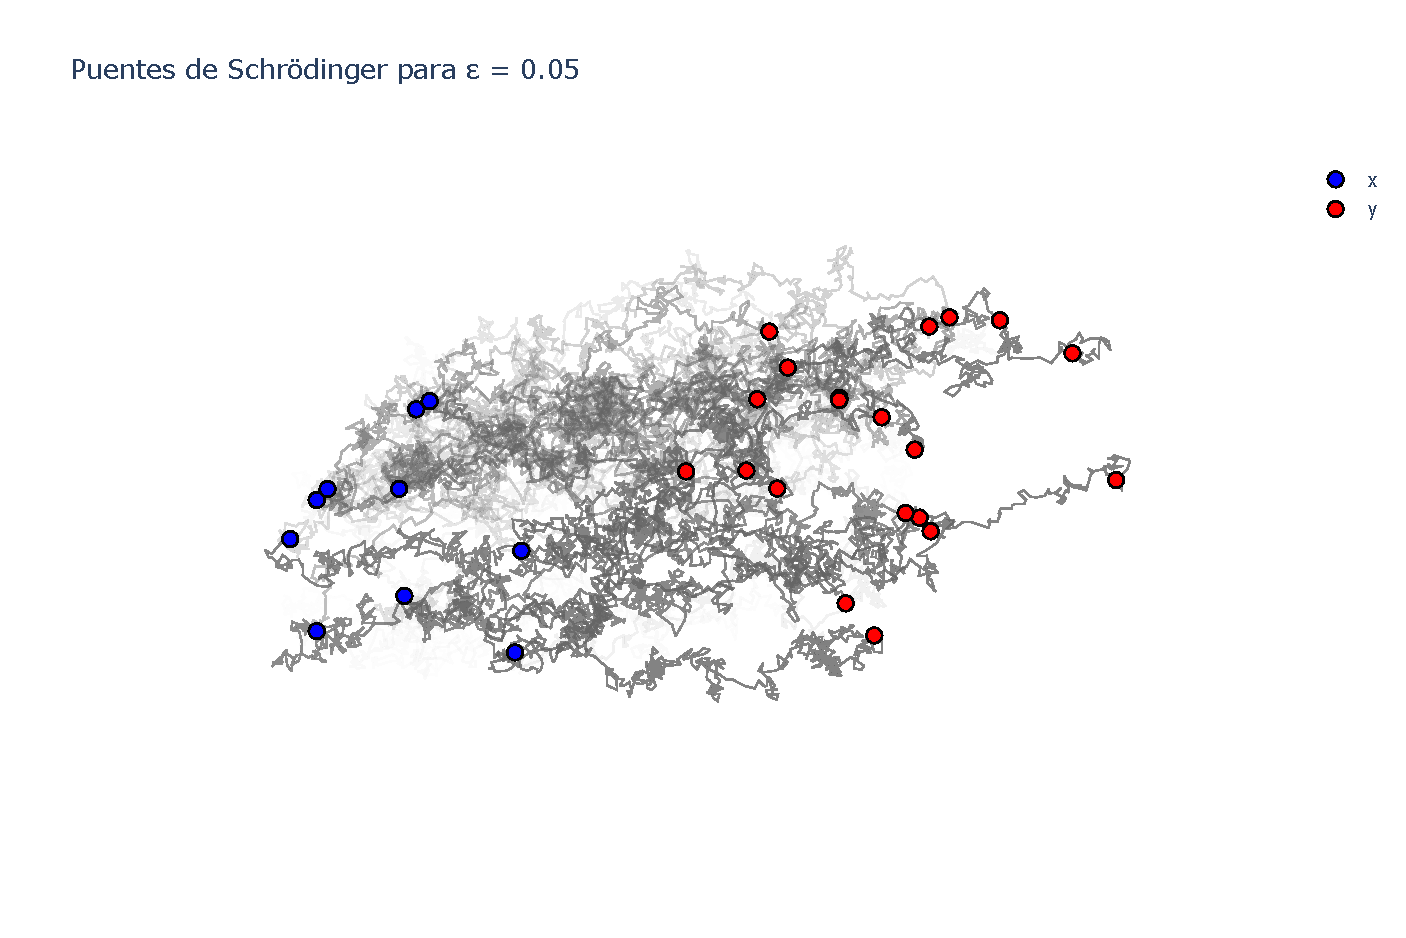
\includegraphics[width=0.7\textwidth]{images/eot_sbp/sbp_solution0.05}
	\caption{Puentes de Schrödinger para distintos valores de $\epsilon$. Se observa como disminuye la aleatoriedad del plan de transporte estocástico cuando disminuye $\epsilon$. El código que genera estas imágenes se encuentra en el archivo \texttt{sbp.ipynb}.}
	\label{fig:sbp}
\end{figure}


\subsection{Formulación de Brenamou-Brenier para el problema de Schrödinger}
\label{eot_sbp/dynamic/schrodinger_equations}

La interpretación fluidodinámica que se le dio al problema de transporte óptimo en el \autoref{ot} puede ser generaliza al problema del puente de Schrödinger de forma natural. Recordando que la dinámica que se optimiza en la formulación de Benamou-Brenier \eqref{eq:benamou_brenier} es determinista, en esta nueva formulación se considera un proceso estocástico de la forma

\begin{equation*}
	\d x_t = v(x_t,t)\d t + \sigma\d w_t, \quad \sigma>0\text{ constante},
\end{equation*}

donde este nuevo sistema dinámico puede interpretarse como el sistema determinista de Benamou-Brenier con un término de ruido adicional. De esta forma, este nuevo proceso tendrá asociada la siguiente ecuación de Fokker-Planck:

\begin{equation*}
	\frac{\partial\rho}{\partial t} + \nabla\cdot(v\rho) - \frac{\sigma^2}{2}\Delta\rho = 0.
\end{equation*}

Esta ecuación corresponde a la ecuación de transporte con un término adicional que indica la estocasticidad del modelo. Por lo tanto, la formulación estocástica para Benamou-Brenier es la siguiente:

\begin{equation}
	\label{eq:benamou_brenier_sbp}
	\inf_{(\rho,v)} \int_0^1 \int_{\xspace} \norm{v(x,t)}^2 \rho(x,t) \d x\d t
	\quad \text{sujeto a} \quad
	\begin{cases}
		\frac{\partial \rho}{\partial t} + \nabla\cdot(\rho v) - \frac{\sigma^2}{2}\Delta\rho = 0\\
		\rho(\cdot,0) = \rho_0\\
		\rho(\cdot,1) = \rho_1,
	\end{cases}
\end{equation}

donde el único cambio fue cambiar la ecuación de transporte por la ecuación de Fokker-Planck. Notar que cuando $\sigma\to 0$ se recupera la formulación de Benamou-Brenier original.

Para encontrar las condiciones de optimalidad de este problema de control, se puede repetir el mismo procedimiento hecho en la \autoref{ot/dynamic/benamou_brenier}, donde la única diferencia es que se añade un término adicional al lagrangiano del problema, el cual puede ser trabajado mediante la segunda identidad de Green:

\begin{equation*}
	-\frac{\sigma^2}{2}\int_\xspace \lambda\Delta \rho \d x = -\frac{\sigma^2}{2}\cdot 0 -\frac{\sigma^2}{2}\int_\xspace \rho\Delta\lambda\d x.
\end{equation*}

Por lo tanto, el lagrangiano toma la siguiente forma para esta formulación:

\begin{equation*}
	L = \int_\xspace\int_0^1 \parent{\frac{1}{2}\norm{v}^2-\frac{\partial\lambda}{\partial t} - \nabla\lambda\cdot v - \frac{\sigma^2}{2}\Delta\lambda}\rho \d t \d x + \cte.
\end{equation*}

Nuevamente, por condición de primer orden, se tiene que $v^* = \nabla\lambda$ es control óptimo, por lo que 

\begin{align*}
	L = -\int_\xspace\int_0^1 \parent{\frac{\partial\lambda}{\partial t} + {\frac{1}{2}\norm{\nabla\lambda}^2} + \frac{\sigma^2}{2}\Delta\lambda}\rho \d t\d x + \cte.
\end{align*}

Luego, si $\lambda$ satisface la ecuación de Hamilton-Jacobi-Bellman, $\frac{\partial\lambda}{\partial t} + {\frac{1}{2}\norm{\nabla\lambda}^2}+\frac{\sigma^2}{2}\Delta\lambda=0$, entonces $L=\cte$ y cualquier $\rho\in\Gamma(\rho_0,\rho_1)$ minimiza el lagrangiano. En consecuencia, se probó el siguiente para la versión estocástica de Benamou-Brenier:

\begin{prop}
	\label{prop:sbp_sys_pre}
	Si $(\rho^*,\lambda^*)$ es solución del sistema acoplado

	\begin{align*}
		&\frac{\partial\rho}{\partial t} + \nabla\cdot(\rho\nabla\lambda) - \frac{\sigma^2}{2}\Delta\rho= 0\\
		& \frac{\partial\lambda}{\partial t} + {\frac{1}{2}\norm{\nabla\lambda}^2} + \frac{\sigma^2}{2}\Delta\lambda=0,
	\end{align*}

	con condiciones de borde $\parent{\rho(\cdot,0)=\rho_0}\,\wedge\, \parent{\rho(\cdot,1)=\rho_1}$, entonces, $(\rho^*,v^*)$ es solución del problema de Benamou-Brenier estocástico \eqref{eq:benamou_brenier_sbp} con $v^*=\nabla\lambda^*$.

\end{prop}

Notar que la primera ecuación del sistema acoplado es la ecuación de Fokker-Planck de la SDE $\d x_t = v(x_t,t)\d t + \sigma\d w_t$ asociada al transporte, mientras que la segunda ecuación (Hamilton-Jacobi-Bellman) es la que codifica la optimalidad del control. Además, dado que esta formulación de Benamou-Brenier equivale al problema de Schrödinger, se puede considerar que el resultado anterior es un criterio de optimalidad para el problema del puente de Schrödinger dinámico.

\subsubsection{Sistema de Schrödinger}

El sistema acoplado de la \autoref{prop:sbp_sys_pre} para el problema de Schrödinger puede ser transformado en otro sistema acoplado equivalente mediante las transformaciones de Hopf-Cole. Aplicando el cambio de variable $(\lambda,\rho)\to(\phi,\hat\phi)$ definido como

\begin{equation*}
	\phi = \exp\parent{\frac{\lambda}{\sigma^2}}
	\quad
	\hat\phi = \rho\exp\parent{\frac{-\lambda}{\sigma^2}},
\end{equation*}

el sistema de la \autoref{prop:sbp_sys_pre} se reduce a:

\begin{align}
	&\frac{\partial\phi}{\partial t} + \frac{\sigma^2}{2}\Delta\phi = 0\\
	&\frac{\partial\hat\phi}{\partial t} - \frac{\sigma^2}{2}\Delta\hat\phi = 0,
\end{align}

con condiciones de borde $\phi(\cdot,0)\hat\phi(\cdot,0) = \rho_0$ y $\phi(\cdot,1)\hat\phi(\cdot,1) = \rho_1$. Este sistema es conocido como \textit{sistema de Schrödinger} y será el que permitirá ver que los modelos de difusión estudiados en el \autoref{dm} son un caso particular del problema del puente de Schrödinger. Para esto, es necesario generalizar el resultado anterior a una familia más amplia de procesos estocásticos. Si se fija como medida de referencia al proceso $\d x_t = f(x_t,t)\d t + \sigma g(t)\d w_t$, se puede probar la siguiente extensión del resultado anterior (ver \cite{chen2020stochasticcontrolliaisonsrichard} para una demostración):

\begin{prop}
	\label{prop:sbp_system}
	Dado el problema de Schrödinger $\min_{P\in\Gamma(\rho_0,\rho_1)} \KL{P}{R}$ con $R$ la medida de un proceso que resuelve la SDE $\d x_t = f(x_t,t)\d t + \sigma g(t)\d w_t$ (con $\sigma>0$ una constante), entonces

	\begin{equation*}
		\inf_{(\rho,v)} \int_0^1 \int_{\xspace} \norm{v(x,t)}^2 \rho(x,t) \d x\d t
		\quad \text{sujeto a} \quad
		\begin{cases}
			\d x_t = \parent{f(x_t,t) + g(t)v(x_t,t)}\d t + \sigma g(t)\d w_t\\
			\rho(\cdot,0) = \rho_0,\\
			\rho(\cdot,1) = \rho_1,
		\end{cases}
	\end{equation*}

	es la formulación de Benamou-Brenier para este problema de Schrödinger. Más aún, las condiciones de optimalidad para este problema son las siguientes:

	\begin{align*}
		&\frac{\partial\phi}{\partial t} + \frac{\sigma^2}{2}\trace{g^2 \Delta\phi} + \nabla\phi^\top f = 0\\
		&\frac{\partial\hat\phi}{\partial t} - \frac{\sigma^2}{2}\trace{g^2 \Delta\hat\phi} + \nabla\cdot(\hat\phi f)= 0,
	\end{align*}

	donde el control óptimo es $v(x_t,t)=\sigma^2 g(t)\nabla\log\phi(x_t,t)$. Así, fijando $\sigma=1$, la solución $P^*$ del problema de Schrödinger viene dada por la ley de cualquiera de las siguientes SDEs:

	\begin{align*}
		\d x_t = (f+g^2\nabla\log\phi(x_t,t))\operatorname{d} t + g\operatorname{d} w_t,\quad x_0\sim\rho_0\\
		\d x_t = (f-g^2\nabla\log\hat\phi(x_t,t))\operatorname{d} t + g\operatorname{d} w_t,\quad x_1\sim\rho_1
	\end{align*}

\end{prop}

En consecuencia, para resolver el problema del puente de Schrödinger para una SDE de referencia usual, se debe resolver el sistema acoplado de la \autoref{prop:sbp_system} y luego simular el proceso forward (usando $\phi$) o el proceso backward (usando $\hat\phi$) para tener una simulación del proceso $P^*$ que resuelve el problema de Schrödinger.

\subsubsection{Problema de Schrödinger como generalización de los modelos de difusión}

Para el entrenamiento de un modelo de difusión a tiempo continuo, el proceso de difusión por lo general debe tener una forma muy simple (p.g. lineal) para poder computar la función de score $\score{x_t}{p(x_t|x_0)}$ de forma cerrada, lo cual muchas veces limita la aplicabilidad de este tipo de modelos. Para concluir este trabajo, se verá un último resultado que permite entrenar un modelo para el problema de Schrödinger mediante verosimilitud. Este método, al igual que los modelos de difusión, permite realizar transporte óptimo en alta dimensión y de manera eficiente. Además, al ser un resultado teórico en el continuo, no se ve afectado por la elección del solver usado.

Se comenzará con el siguiente resultado, el cual transforma el sistema de PDEs acoplado de la \autoref{prop:sbp_system} en un sistema acoplado de SDEs:

\begin{teo}[Feynman-Kac para el problema de Schrödinger]
	\label{teo:feynman_kac_sbp}

	Sea
	\begin{align*}
		&\d x_t = (f+gz_t)\d t + g\d w_t\\
		&\d y_t = \frac{1}{2} z_t^\top z_t \d t + z_t^\top \operatorname{d} w_t\\
		&\d \hat y_t = \parent{\frac{1}{2}\hat z_t^\top \hat z_t^ + \nabla\cdot(g\hat z_t + f) + \hat z_t^\top z_t}\operatorname{d} t + \hat z_t^\top \operatorname{d} w_t,
	\end{align*}

	un sistema acoplado con condiciones de borde $x_0\sim\delta_{x_0}$ e $y_1+\hat y_1 = \log \rho_1(x_1)$. Entonces, las relaciones de Feynman-Kac entre el sistema de PDEs de la \autoref{prop:sbp_system} y este nuevo sistema de SDEs son las siguientes:

	\begin{align*}
		y_t &= \log \phi(x_t,t),\quad z_t = g\nabla\log\phi(x_t,t)\\
		\hat y_t &= \log \hat\phi(x_t,t),\quad \hat z_t = g\nabla\log\hat\phi(x_t,t).
	\end{align*}

	Además, se tiene que $y_t + \hat y_t = \log p(x_t)$, $\forall t\in[0,1]$, donde $p$ es la densidad de la solución del problema de Schrödinger de la \autoref{prop:sbp_system}.
	
\end{teo}

En consecuencia, es posible recuperar los procesos forward y backward de la \autoref{prop:sbp_system} (que corresponden a la solución del problema de Schrödinger hacia adelante y hacia atrás en el tiempo) a partir de $z_t$ y $\hat z_t$. Para entrenar estos modelos, se utilizará el siguiente resultado, cuya demostración se puede encontrar en \cite{chen2023likelihoodtrainingschrodingerbridge}:

\begin{teo}[verosimilitud para el problema de Schrödinger]
	\label{teo:sbp_likelihood}
	Para un modelo $(z_t,\hat z_t)$ del problema de Schrödinger (de acuerdo a la \autoref{teo:feynman_kac_sbp}), la verosimilitud de un punto $x_0\in\xspace$ puede ser escrita como:

\begin{equation}
	\label{eq:sbp_likelihood}
	\log p(x_0) = \E{}{\log p(x_1)} - \int_0^1 \E{}{\frac{1}{2}\norm{z_t + \hat z_t}^2 + \nabla\cdot\parent{\sigma_t \hat z_t - f}} \d t
\end{equation}

\end{teo}

Por lo tanto, entrenando un modelo paramétrico según \eqref{eq:sbp_likelihood} para $z_t$ y otro para $\hat z_t$, es posible entrenar un modelo neuronal de forma eficiente para el problema de Schrödinger. Para las divergencias dentro de la función objetivo se puede usar un estimador eficiente como el estimador de Hutchinson. En la \autoref{fig:eot_sbp/sbp_images} se pueden ver muestras generadas utilizando este enfoque.

Notar que la función objetivo \eqref{eq:sbp_likelihood} colapsa a la función objetivo de un modelo de difusión cuando $(z_t,\hat z_t)=(0,gs_\theta)$ (ver \autoref{teo:dm_likelihood}). Esto ocurre cuando la medida de referencia $R$ por si sola es capaz de alcanzar la distribución $\rho_1$ ya que, en este caso, no hay que hacer un esfuerzo adicional para alcanzar $\rho_1$, por lo que $z_t=0$ y $\hat z_t$ colapsa a $gs_\theta$.

\insertimage{eot_sbp/sbp_images}{0.8}{Imágenes generadas utilizando el enfoque del \autoref{teo:sbp_likelihood} sobre los datasets MNIST, CelebA y CIFAR-10. Imagen obtenida desde \cite{chen2023likelihoodtrainingschrodingerbridge}.}